
\documentclass[11pt]{article}
\usepackage[top=0.7in, left=1in, right=1in, bottom=1in]{geometry}
\usepackage{amsmath}
\usepackage{graphicx}
\usepackage{microtype}
\usepackage{tikz-cd}
\usepackage{enumitem}
\usepackage{booktabs}
\usepackage{tikz}
\usepackage{tcolorbox}
\usepackage{siunitx}  
\usetikzlibrary{arrows.meta, positioning}

\setlength{\parindent}{0pt}
\setlength{\parskip}{0.5\baselineskip}


\title{\textbf{R-Peak Detection in ECG Using Wavelet Transform and K-Means Clustering}}
\author{María Isabel Sánchez-O'Mullony Martínez}


\begin{document}


\maketitle


\section{Introduction}\label{sec:intro}
This report describes the design and implementation of an R-peak detection algorithm for electrocardiogram (ECG) signals.

R-peak detection is a well-studied problem, and numerous methods have been proposed in the literature. A comprehensive review by H.\ Dogan and R.\ O.\ Dogan (2023)~\cite{dogan_comprehensive_2023} surveys the most prominent techniques and evaluates their relative performance.

Following a thorough review of existing approaches, the method proposed by Xia et al.\ (2015)~\cite{xia_quick_2015} was selected as the foundation for this implementation and subsequently extended. The pipeline consists of three main stages: a wavelet-based preprocessing stage that enhances QRS complexes, computation of an absolute-slope feature to capture rapid signal changes, and segmented K-means clustering to identify QRS regions. R-peaks are then extracted as local maxima within each identified region, followed by a refractory filter consistent with physiological heart-rate limits.

Wavelet transforms are widely used for R-peak detection due to their ability to localise signal features in both time and frequency. When combined with K-means clustering, this approach is computationally efficient, straightforward to implement, and robust to noise, achieving a reported accuracy of approximately 99.7\%.

The implementation was evaluated on the MIT-BIH Arrhythmia Database~\cite{mitbih_physionet}, consistent with the original paper.

Finally, to evaluate real-world adaptability, the modular pipeline is extended to the PhysioNet ECGRDVQ pharmacological database. The algorithm is benchmarked against the classical Pan-Tompkins method, revealing a significant clinical advantage in mitigating T-wave over-sensing caused by drug-induced repolarization abnormalities.


\section{R-Peaks}\label{sec:r-peaks}

A typical ECG signal comprises three principal segments: the P-wave, the QRS complex, and the T-wave. Each segment reflects a distinct phase of cardiac electrical activity and provides clinically valuable information about the state of the cardiovascular system.

The QRS complex is the most diagnostically significant segment, corresponding to the depolarisation of the right and left ventricles.

\begin{figure}[htbp]
    \centering
    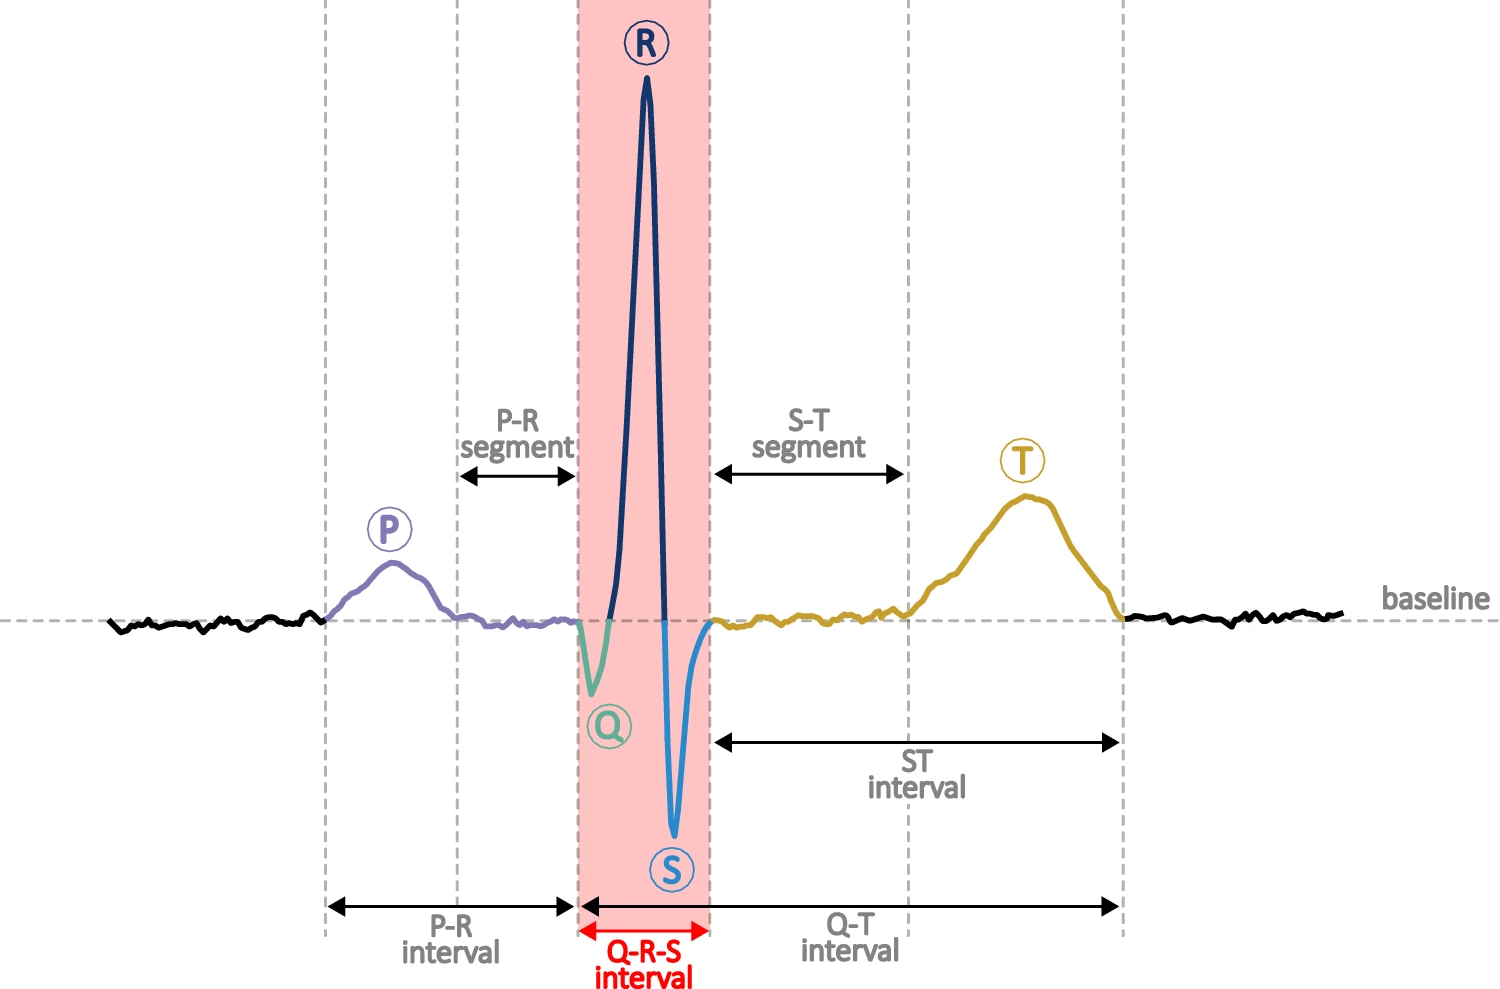
\includegraphics[width=0.8\textwidth]{imgs/R-peaks.png}
    \caption{Segments of an ECG signal~\cite{dogan_comprehensive_2023}}
    \label{fig:segments}
\end{figure}


\section{Methodology}\label{sec:method}

The detection pipeline follows the method proposed by Xia et al.~\cite{xia_quick_2015}. ECG recordings from the MIT-BIH Arrhythmia Database are first loaded and passed through a wavelet decomposition stage, which attenuates noise and removes unwanted frequency components to produce a clean signal. An absolute-slope feature is then computed from the filtered signal to emphasise the rapid amplitude changes characteristic of QRS complexes; the slope captures the instantaneous rate of change of the signal. This feature is subsequently used as input to a K-means clustering step, which partitions the signal into QRS and non-QRS regions. R-peaks are finally extracted as local maxima within each identified QRS region, as illustrated in Figure~\ref{fig:method}. The following sections describe each stage of the pipeline in detail.

\begin{figure}[htbp]
    \centering
    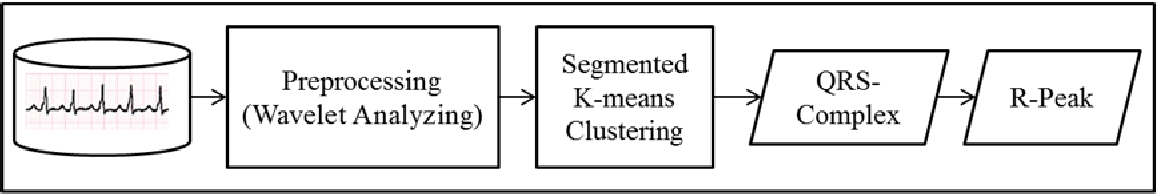
\includegraphics[width=1\textwidth]{imgs/Method.png}
    \caption{Overview of the detection pipeline~\cite{xia_quick_2015}}\label{fig:method}
\end{figure}


\subsection{Modular Pipeline Architecture}\label{sec:modular}
To ensure the algorithm is robust and adaptable to various datasets, the implementation was refactored into a highly modular pipeline consisting of distinct stages:

\begin{enumerate}[label=\arabic*.]
    \item \textbf{Preprocessing:} Applies Wavelet Denoising (using \texttt{sym8}) and a dynamic Polarity Correction module to orient the QRS complexes positively.
    \item \textbf{Feature Extraction:} Computes the absolute gradient slope of the cleaned signal to emphasize high-frequency variations characteristic of R-peaks.
    \item \textbf{QRS Masking:} Segments the signal into 60-second windows and applies K-Means clustering ($k=2$) to the gradient features, isolating the QRS regions from the background.
    \item \textbf{Peak Extraction \& Refractory Filtering:} Identifies the local maximum within each QRS region. A physiological refractory filter of \SI{200}{ms} is then applied, retaining the highest amplitude peak if multiple detections occur too closely.
    \item \textbf{Evaluation:} An independent module compares detected peaks against annotated ground truth files, calculating metrics such as Sensitivity (Se) and Positive Predictive Value (PPV) within a defined tolerance window (e.g., \SI{150}{ms}).
\end{enumerate}


\section{Exploratory Analysis}\label{sec:exploratory}

Before designing the detector, it is important to understand the structure and characteristics of the data. In this experiment, 30-minute ECG recordings sampled at 360\,Hz are used. The MIT-BIH Arrhythmia Database provides expert annotation files that serve two purposes: as a sanity check during development, and as ground truth for quantitative evaluation of detection performance.

Figure~\ref{fig:sample100} shows a time-domain visualisation of sample 100. The upper panel displays the full 30-minute window, in which several abnormal beats are visible as large-amplitude spikes. The two lower panels show shorter segments at increasing resolution; red triangles mark the R-peak annotations provided by the experts. The QRS complexes are clearly distinguishable, with prominent R-peaks and visible P and T waves of smaller amplitude.

\begin{figure}[htbp]
    \centering
    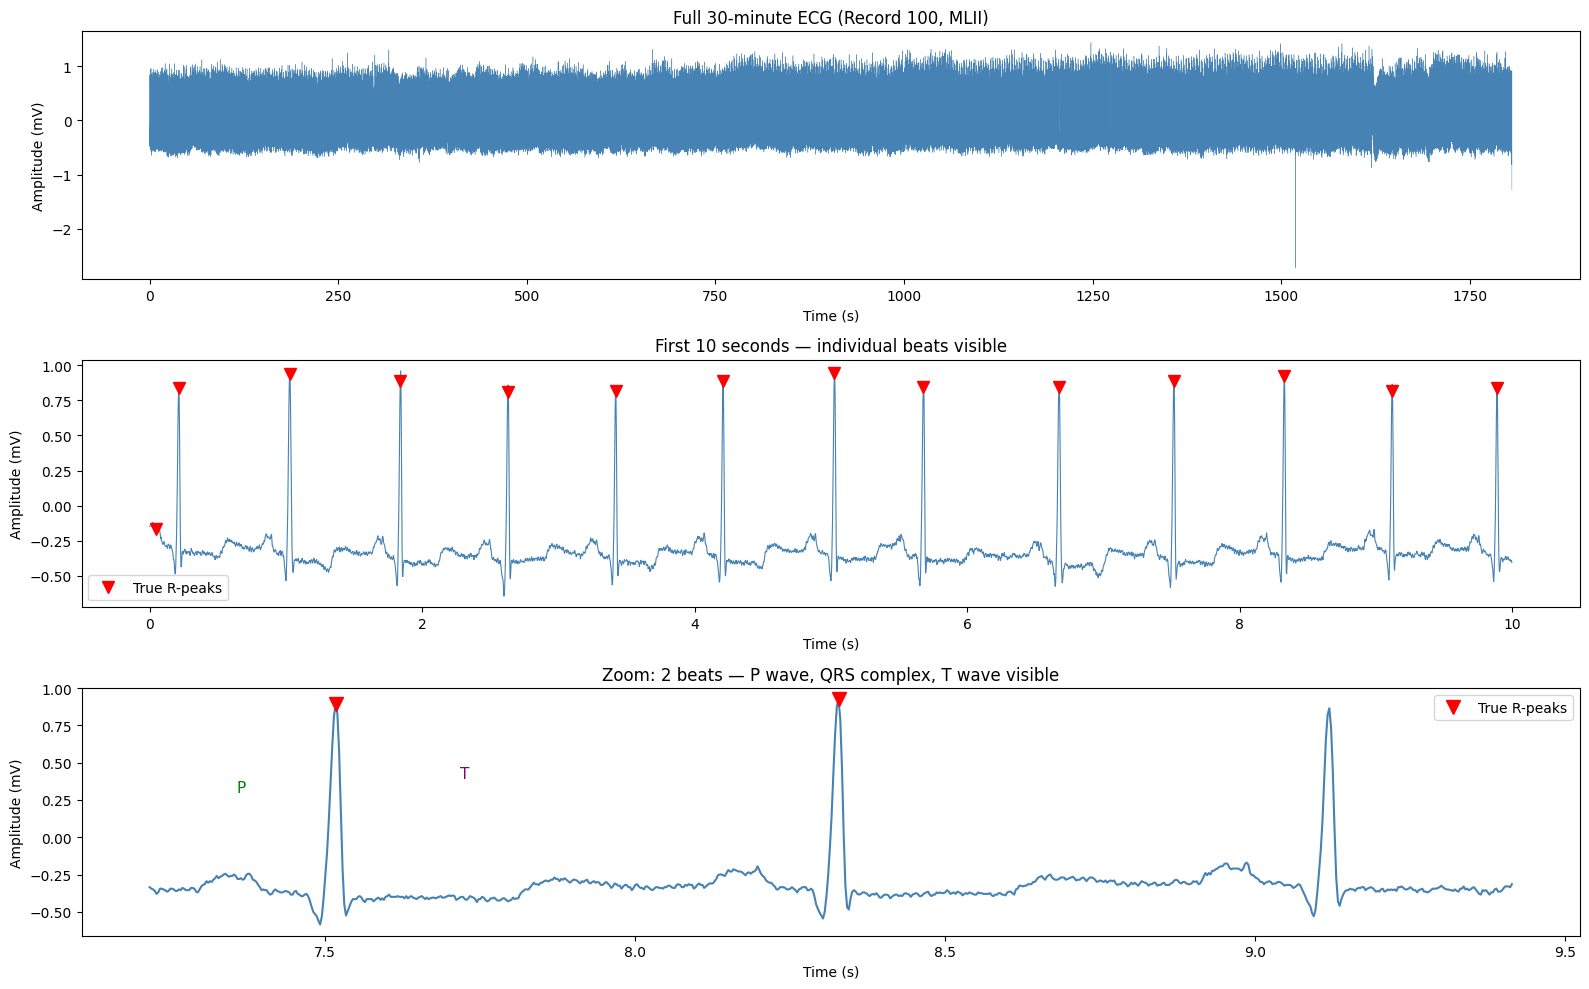
\includegraphics[width=1\textwidth]{imgs/Sample 100.png}
    \caption{Time-domain visualisation of MIT-BIH sample 100.}
    \label{fig:sample100}
\end{figure}

To further characterise the signal, a Fourier Transform was applied to convert the recording from the time domain to the frequency domain. Unlike the time-domain representation, the frequency-domain view reveals how much energy the signal contains at each frequency, without retaining temporal information. A high-frequency component oscillates rapidly, whereas a low-frequency component changes slowly.

Figure~\ref{fig:ft} shows the Fourier magnitude spectrum of the signal, with the three main regions of interest highlighted. The red region corresponds to baseline wander, which arises primarily from respiration and occurs at very low frequencies (below 0.5\,Hz)~\cite{luo_review_2010}. The yellow region marks power-line interference at 50 or 60\,Hz, which in this recording carries negligible energy, indicating low electrical noise. The green region represents the QRS energy concentration band of 5--15\,Hz, where most of the QRS signal power is concentrated~\cite{sharma_qrs_2017}. Although the QRS complex spans a broader bandwidth of up to 50\,Hz~\cite{tereshchenko_frequency_2015}, the bulk of its energy resides in this lower band, making it the primary target for the bandpass filtering stage of the detection pipeline. Table~\ref{tab:ecg-components} summarises the frequency characteristics of the main ECG components and noise sources.

\begin{figure}[htbp]
    \centering
    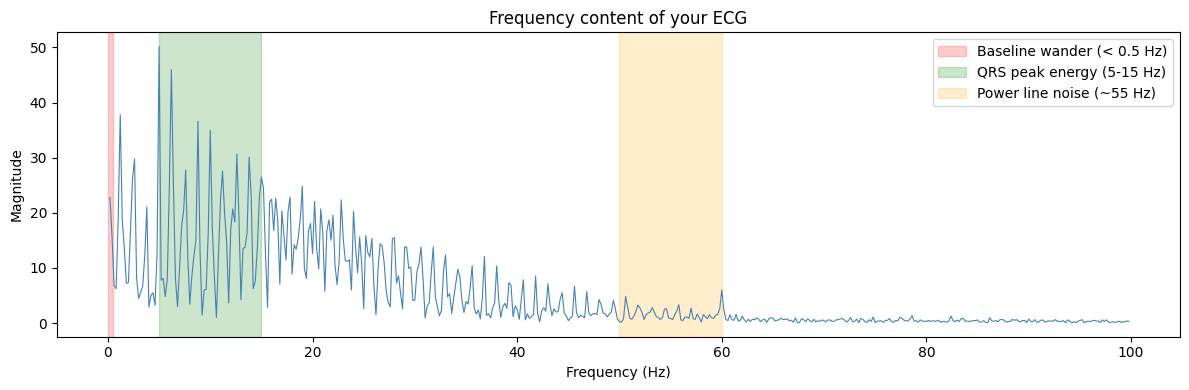
\includegraphics[width=1\textwidth]{imgs/Fourier Transform.png}
    \caption{Fourier magnitude spectrum of MIT-BIH sample 100.}
    \label{fig:ft}
\end{figure}

\begin{table}[htbp]
    \centering
    \caption{Frequency characteristics of ECG signal components and noise sources~\cite{luo_review_2010, tereshchenko_frequency_2015, xie_computational_2020}}
    \label{tab:ecg-components}
    \begin{tabular}{lll}
        \toprule
        \textbf{Component} & \textbf{Freq.\ Range} & \textbf{Physical Cause} \\
        \midrule
        Baseline wander   & 0.05--0.5\,Hz   & Patient movement, electrode contact     \\
        QRS complex       & 8--50\,Hz       & Rapid ventricular depolarisation        \\
        EMG (muscle)      & 50--150\,Hz     & Electromyographic interference          \\
        Power line noise  & 50 or 60\,Hz    & Electrical interference (PLI)           \\
        \bottomrule
    \end{tabular}
\end{table}


\section{Wavelet Decomposition}\label{sec:wavelet}

With the frequency characteristics of the ECG signal established, the signal can now be decomposed into frequency layers to better understand its structure. The ECG signal is decomposed into multiple levels using the discrete wavelet transform (DWT), with each level capturing a specific frequency band. In total, 8 decomposition levels are used.

The number of levels is determined by the sampling frequency of the signal and the lowest frequency that needs to be isolated. ECG signals from the MIT-BIH Arrhythmia Database are sampled at $f_s = 360$\,Hz. The maximum representable frequency in a digital signal is half the sampling rate, known as the Nyquist frequency~\cite{tereshchenko_frequency_2015, zidelmal_qrs_2012}:

$$f_\mathrm{N} = \frac{f_s}{2} = 180\,\text{Hz}.$$

At each decomposition level $n$, the detail coefficients capture an approximate frequency band defined by:

$$f_\text{low}(n) = \frac{f_s}{2^{n+1}}, \qquad f_\text{high}(n) = \frac{f_s}{2^{n}}.$$

The number of levels is chosen to answer the question: \textit{what is the lowest frequency that needs to be isolated?} Decomposing to level 8 ensures that the approximation coefficients capture frequencies below approximately 0.7\,Hz, which fully encompasses the baseline wander band (below 0.5\,Hz). The resulting frequency bands for $f_s = 360$\,Hz are summarised in Table~\ref{tab:wavelet-levels}.

\begin{table}[htbp]
    \centering
    \caption{Wavelet decomposition levels and their corresponding frequency bands for $f_s = 360$\,Hz~\cite{sharma_qrs_2017, zidelmal_qrs_2012}.}
    \label{tab:wavelet-levels}
    \begin{tabular}{llll}
        \toprule
        \textbf{Level} & \textbf{Freq.\ Band (Hz)} & \textbf{Content} & \textbf{Action} \\
        \midrule
        cA8 & 0.00 -- 0.70   & Baseline drift          & Remove \\
        cD8 & 0.70 -- 1.41   & Slow baseline variation & Keep   \\
        cD7 & 1.41 -- 2.81   & Very low frequency ECG  & Keep   \\
        cD6 & 2.81 -- 5.62   & Low frequency ECG       & Keep   \\
        cD5 & 5.62 -- 11.25  & QRS energy              & Keep   \\
        cD4 & 11.25 -- 22.50 & QRS energy              & Keep   \\
        cD3 & 22.50 -- 45.00 & QRS high-frequency edge & Keep   \\
        cD2 & 45.00 -- 90.00 & High-frequency noise    & Remove \\
        cD1 & 90.00 -- 180.00 & High-frequency noise   & Remove \\
        \bottomrule
    \end{tabular}
\end{table}

The levels of primary interest are cD4 and cD5, which correspond to the 5--22.5\,Hz band where the bulk of QRS energy is concentrated~\cite{sharma_qrs_2017, zidelmal_qrs_2012}. Since the QRS complex spans a broader bandwidth of up to 50\,Hz~\cite{tereshchenko_frequency_2015}, levels cD6, cD7, and cD8 are retained as well to preserve the full QRS morphology. At the other extreme, cA8, cD1, and cD2 are discarded, removing baseline drift and high-frequency noise respectively.

Level cD3 (22.5--45\,Hz) deserves particular attention. Although this band lies above the core QRS energy region, Figure~\ref{fig:wavelet} shows that cD3 retains a noticeable beat structure, indicating that sharp QRS edges contribute energy at these frequencies. Removing cD3 would therefore attenuate the high-frequency components of the QRS spike, reducing peak amplitude from approximately 1.2\,mV to 0.95\,mV and making the slope contrast between QRS complexes and T-waves smaller — which in turn makes the subsequent K-Means separation harder. Including cD3 is therefore the conservative and preferred choice.

\begin{figure}[htbp]
    \centering
    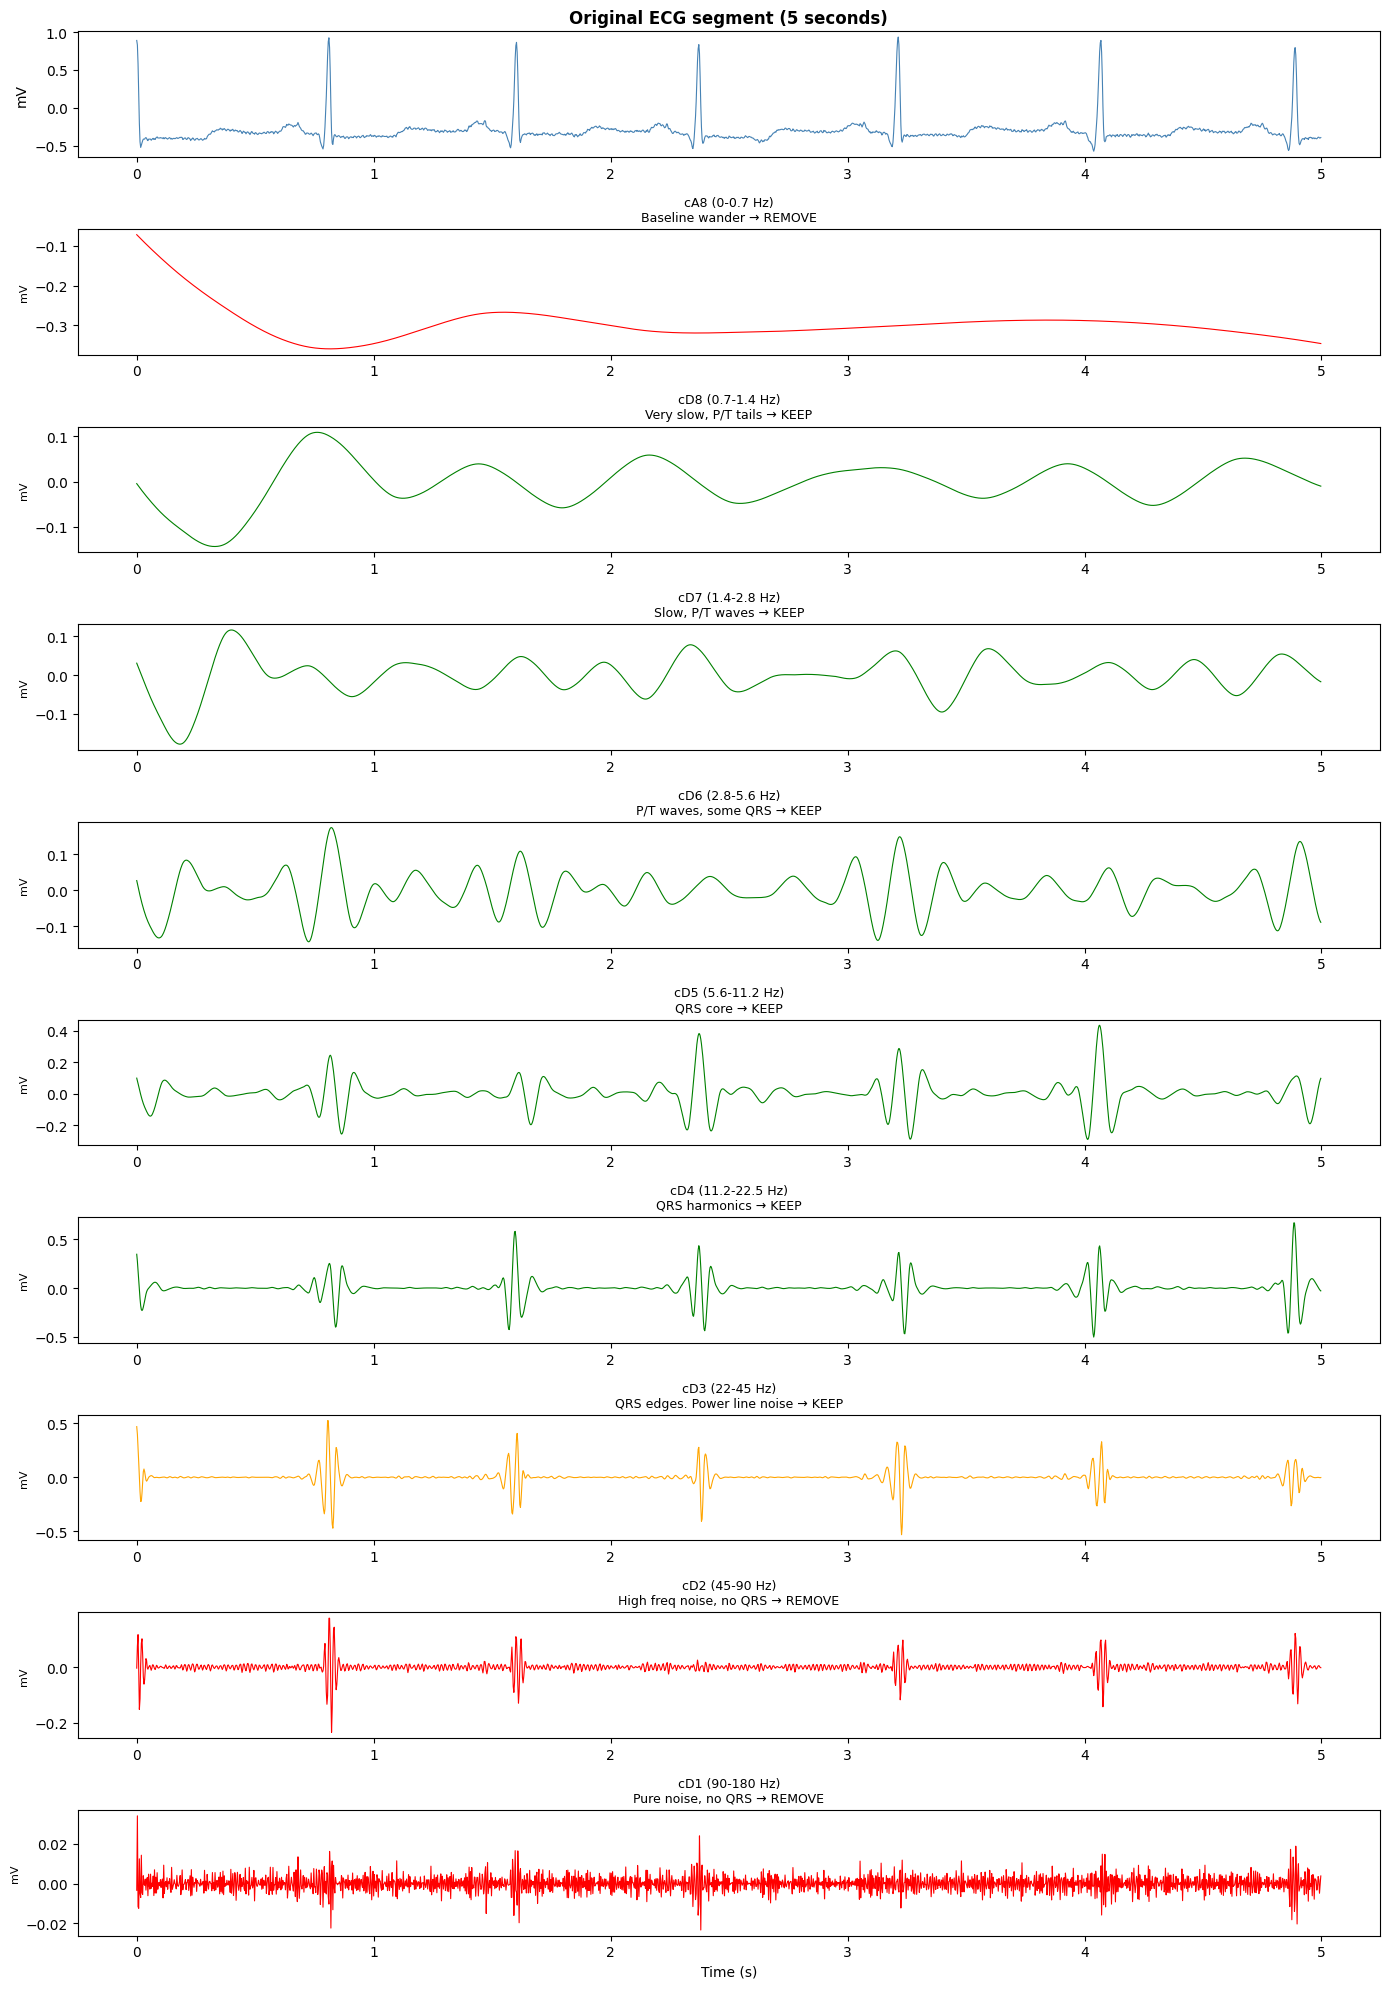
\includegraphics[width=0.88\textwidth]{imgs/Wavelet.png}
    \caption{Wavelet decomposition of the ECG signal across all 8 levels.}
    \label{fig:wavelet}
\end{figure}

It is worth noting that the wavelet reconstruction does not need to produce a perfect, QRS-only signal. Its purpose is simply to make QRS complexes the dominant, highest-slope feature in the signal — K-Means clustering handles the segmentation afterwards. This leads to two important design trade-offs:

\begin{itemize}
    \item \textbf{Over-filtering} (retaining too few levels) risks weakening QRS peaks, reducing the slope contrast between QRS and T-waves and making K-Means separation less reliable.
    \item \textbf{Under-filtering} (retaining too many levels) leaves P and T waves present in the signal, but their slopes remain substantially smaller than those of QRS complexes, so K-Means can still separate them cleanly.
\end{itemize}

Figures~\ref{fig:clean} and~\ref{fig:clean2} compare the two reconstruction choices. Each figure shows the original signal (blue), the reconstructed clean signal (green), and the removed components (red). A key diagnostic check is that the red panel should contain no visible QRS spikes — any QRS energy in the removed component represents signal loss that would degrade detection performance.

\begin{figure}[htbp]
    \centering
    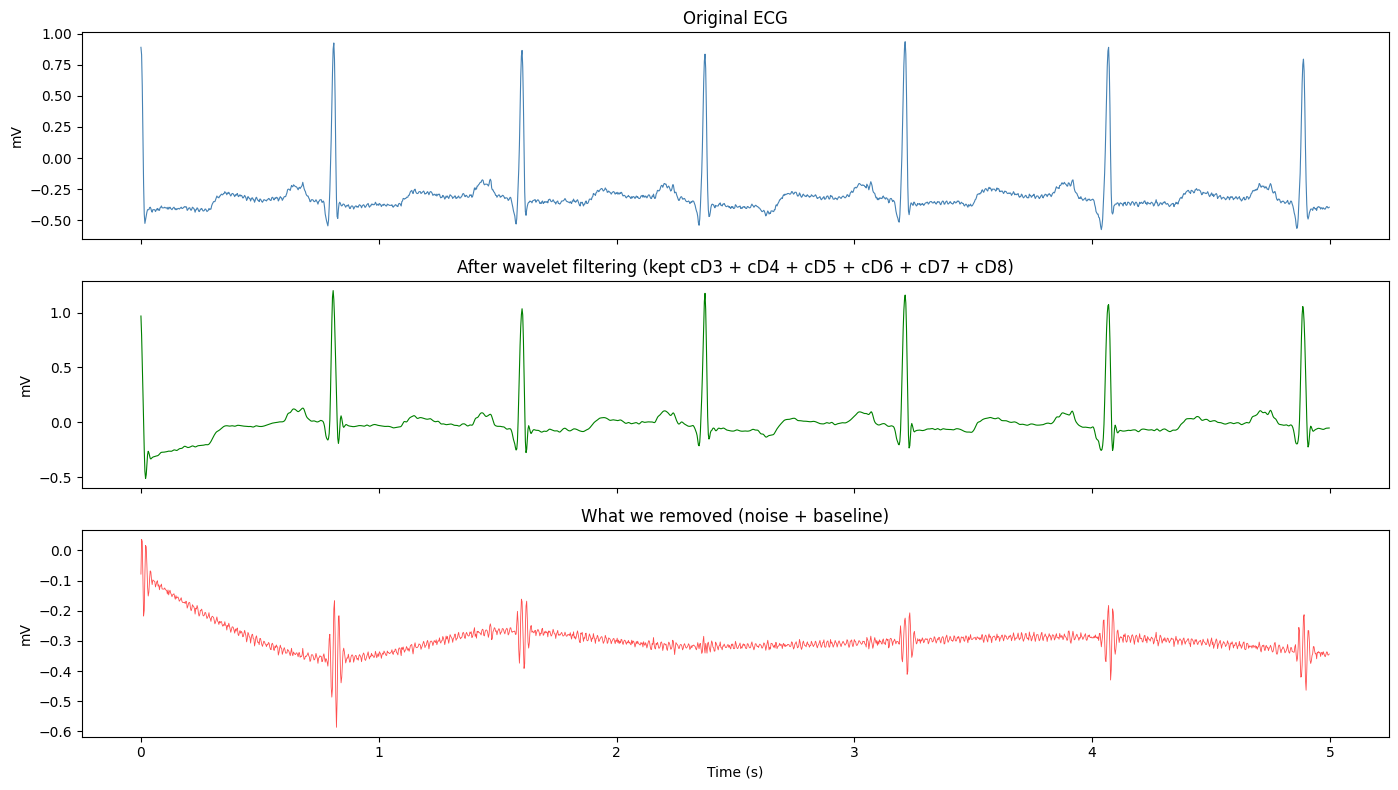
\includegraphics[width=1\textwidth]{imgs/Clean signal.png}
    \caption{Reconstructed signal using levels cD3--cD8.}
    \label{fig:clean}
\end{figure}

\begin{figure}[htbp]
    \centering
    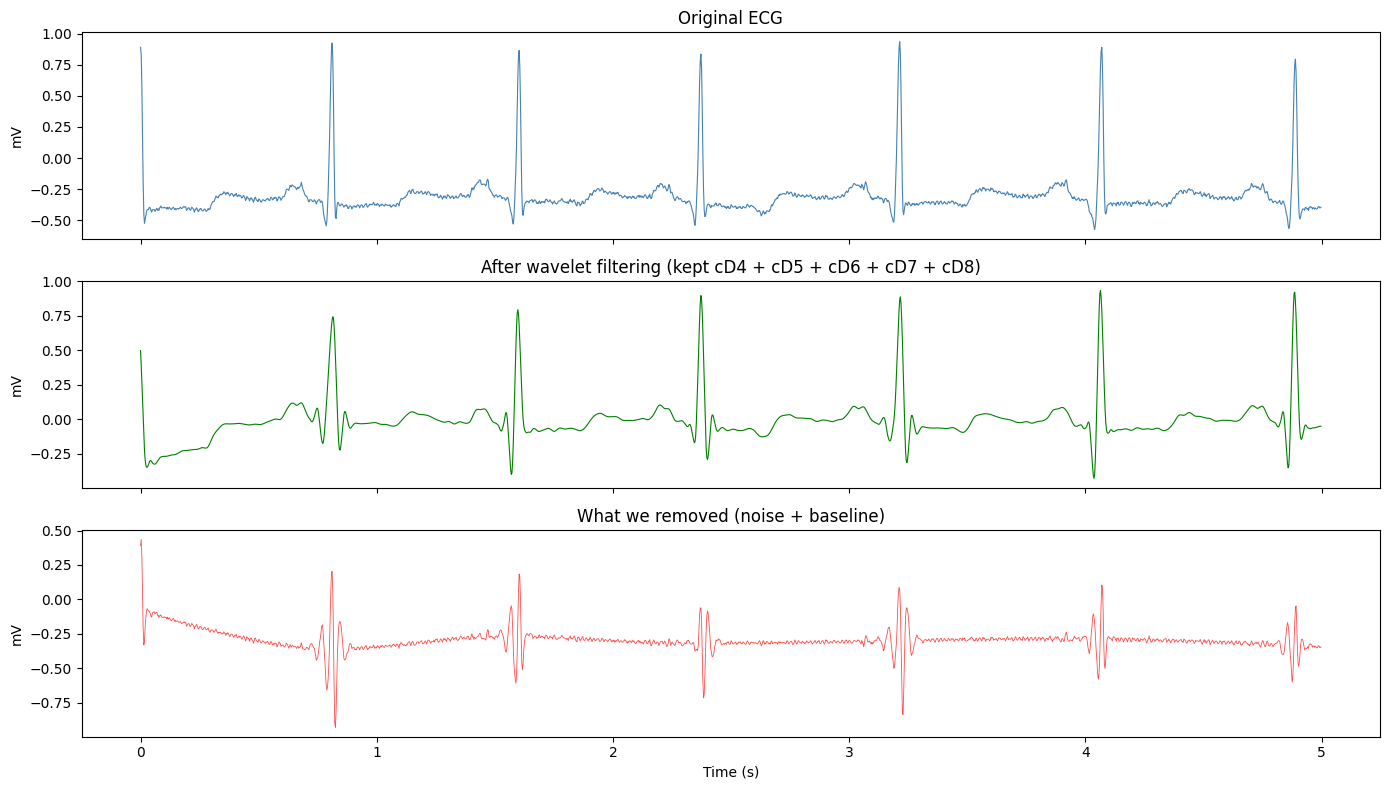
\includegraphics[width=1\textwidth]{imgs/Clean signal 2.png}
    \caption{Reconstructed signal using levels cD4--cD8, excluding cD3.}
    \label{fig:clean2}
\end{figure}

While small QRS-shaped blips remain visible in the red panel even with cD3 included, this is acceptable and unavoidable — the corresponding frequency band is too contaminated by noise to retain without degrading signal quality.


\section{QRS Region Detection via Absolute Slope and Segmented K-Means}\label{sec:slope-kmeans}

The key insight from Xia et al.\ (2015)~\cite{xia_quick_2015} is to use the local slope of the signal rather than its amplitude as the primary discriminating feature. Unlike traditional threshold-based methods that attempt to locate R-peaks directly from amplitude, this approach first identifies the QRS region using slope information, and then extracts the R-peak as the local maximum within that region. The data is divided into 1-minute segments, and K-Means clustering is applied to the absolute slope values within each segment independently. The algorithm groups slope values into two clusters: one capturing the high-intensity fluctuations characteristic of QRS complexes, and one capturing the lower-intensity background activity of P and T waves. Points belonging to the higher-slope cluster are labelled as part of the QRS region.


\subsection{Absolute Slope}\label{subsec:slope}

After wavelet denoising, the clean signal still contains multiple types of deflections: the prominent  QRS complexes and the smaller, broader P and T waves. A naïve approach would be to apply a global amplitude threshold — that is, to declare any peak above some fixed value $X$\,mV as an R-peak. However, this strategy is fundamentally fragile: ECG amplitudes vary significantly across patients, across leads, and even within the same recording as a patient changes posture or activity level. Any fixed threshold would require manual tuning for every recording, which is neither practical nor robust.

The slope offers a more principled solution. Rather than asking \textit{how tall} a peak is, it asks \textit{how fast} the signal is changing. This distinction is reliable regardless of absolute amplitude: QRS complexes, driven by rapid ventricular depolarisation~\cite{dogan_comprehensive_2023}, produce the steepest signal transitions in the ECG, while P and T waves change much more gradually. The speed of change is therefore a more stable separator than amplitude alone.

The simplest approximation of the slope is the forward difference, which estimates the rate of change using only the next sample:

$$\text{slope}(k) = \text{data}(k+1) - \text{data}(k)$$

In this implementation, the central-difference approximation is used instead, via the gradient, which considers both neighbouring samples:

$$\text{gradient}(k) = \frac{\text{data}(k+1) - \text{data}(k-1)}{2}$$

This is marginally smoother than the forward difference, since it reduces sensitivity to isolated sample noise by looking both forward and backward. The absolute slope is then the magnitude of the gradient:

$$\text{abs\_slope}(k) = |\text{gradient}(k)|$$

Figure~\ref{fig:slope} shows the result of this transformation. A notable characteristic is that each QRS complex produces \textit{two} spikes in the absolute slope rather than one. This arises from the morphology of the QRS complex itself: as illustrated in Figure~\ref{fig:segments}, the rising edge of the R-peak produces a large positive slope, while the falling edge into the S-wave produces a large negative slope. Taking the absolute value folds both edges upward, resulting in a double spike at each QRS location. This is in fact desirable — it flags the entire QRS region as high-slope rather than only one edge, making the subsequent clustering step more robust.

\begin{figure}[htbp]
    \centering
    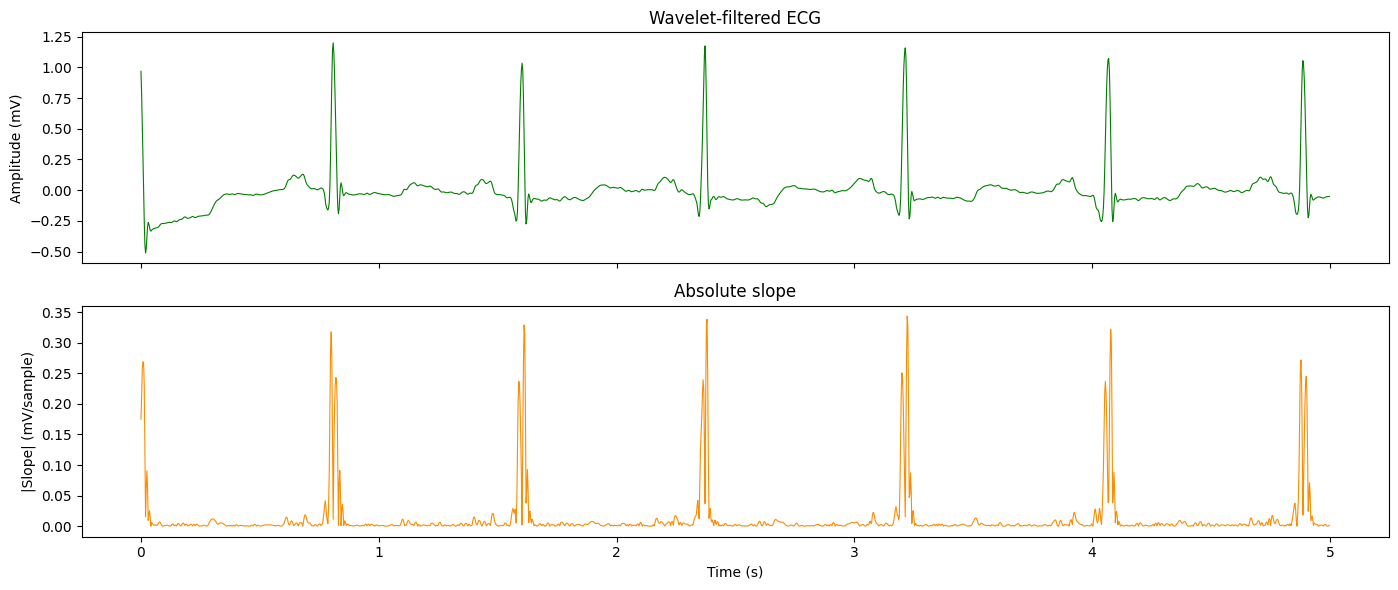
\includegraphics[width=1\textwidth]{imgs/Absolute Slope.png}
    \caption{Absolute slope of the wavelet-filtered ECG signal.}
    \label{fig:slope}
\end{figure}


\subsection{Segmented K-Means}\label{subsec:k-means}

With the absolute slope computed, the task reduces to separating high-slope samples (QRS edges) from low-slope samples (baseline, P waves, T waves). K-Means clustering with $k=2$ is therefore well suited to this task: it partitions the slope values into exactly two groups by minimising the within-cluster variance, without requiring any manually chosen threshold~\cite{xia_quick_2015}.

A naïve approach would apply K-Means to the entire 30-minute signal at once. This fails because QRS amplitudes — and therefore slopes — drift over the course of a recording. If a patient becomes more active partway through, QRS amplitudes may increase substantially, causing the global centroids to shift upward. Early beats with lower slopes would then fall into the non-QRS cluster even though they are genuine QRS complexes. A global clustering cannot adapt to these slow amplitude changes.

Xia et al.~\cite{xia_quick_2015} address this by applying K-Means independently to 1-minute segments. Each segment computes its own pair of centroids, adapting to the local amplitude characteristics of that window. This is the key practical innovation that makes the algorithm robust over long recordings. With a 30-minute signal sampled at $f_s = 360$\,Hz, each segment contains $1 \times 60 \times 360 = 21{,}600$ samples, and the clustering is repeated 30 times in total.

Within each segment, K-Means produces two cluster labels. The QRS cluster is identified as the one with the higher centroid value, since QRS edges always produce larger slopes than background activity. 

Formally, let $\mu_0$ and $\mu_1$ denote the two centroids; the cluster with the larger centroid is designated as the \emph{QRS} cluster:

$$c_{\text{QRS}} = \arg\max_{j \in \{0,1\}} \mu_j$$

All samples assigned to this cluster are marked as QRS candidates in a binary mask \(\text{qrs\_mask}[k] \in \{0,1\}\). Figure~\ref{fig:k-means} shows the outcome of this step for the first 10 seconds of the recording. The upper panel shows the wavelet-filtered ECG for reference; the middle panel shows the absolute slope with QRS regions highlighted in blue; and the lower panel overlays the identified QRS regions (red) on the filtered ECG.

\begin{figure}[htbp]
    \centering
    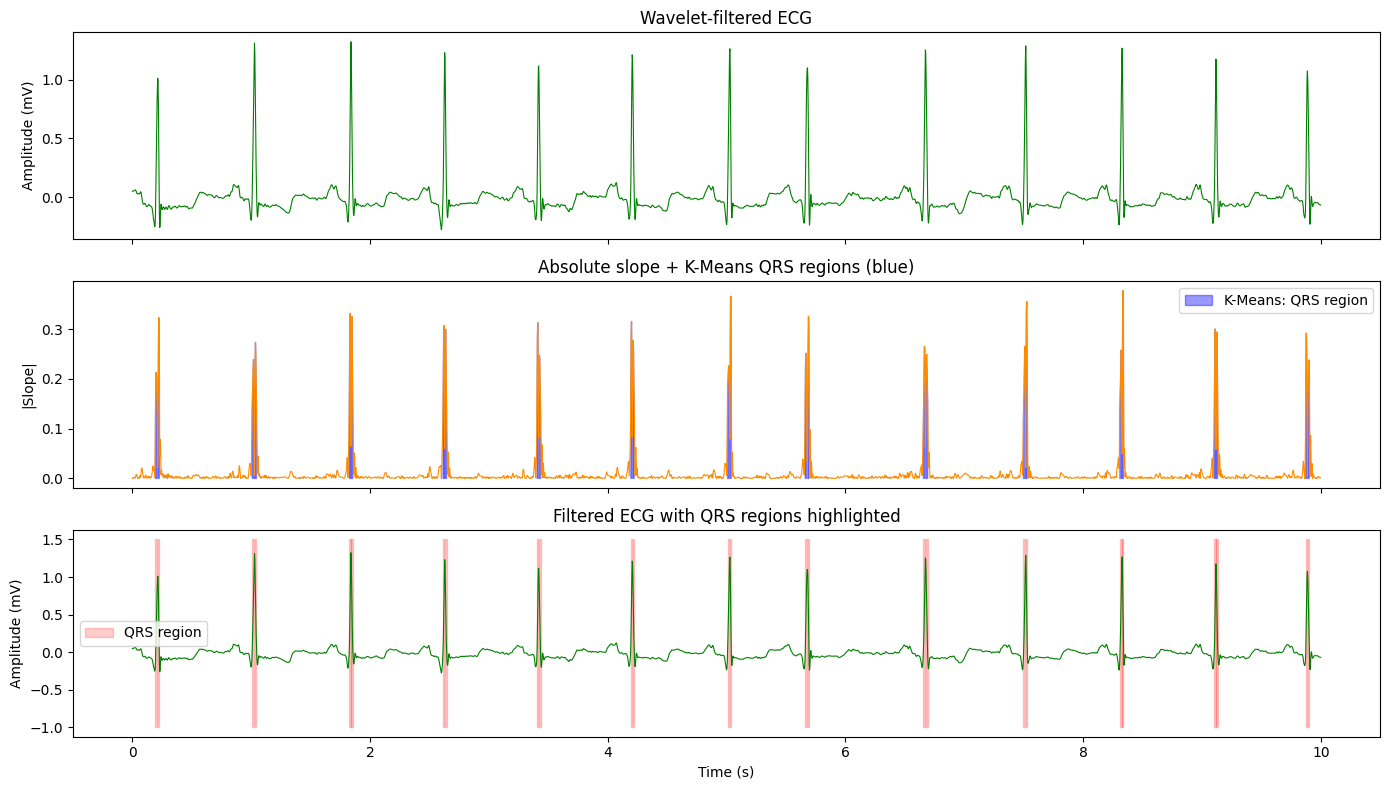
\includegraphics[width=1\textwidth]{imgs/K-Means.png}
    \caption{Result of segmented K-Means clustering.}
    \label{fig:k-means}
\end{figure}

In the middle panel, every QRS slope spike gets correctly shaded blue. Notice the shading captures the double-spike pattern (rising + falling edge) as one connected region, mentioned in Subsection~\ref{subsec:slope}. In the lower panel, each red column sits precisely on top of a QRS spike. The regions look narrow and well-localised, correctly capturing 
each QRS complex without bleeding into the neighbouring P or T waves.


It is worth emphasising that the output of this stage is not yet a set of R-peak locations — it is a set of QRS \textit{regions}. The R-peak is subsequently extracted as the local maximum of the filtered ECG within each identified region, as described in Subsection~\ref{subsec:extraction}.


\subsection{R-Peak Extraction}\label{subsec:extraction}

As described in Subsection~\ref{subsec:k-means}, the output of the segmented K-Means stage is a binary QRS mask in which each sample is labelled as QRS (1) or non-QRS (0). The goal of R-peak extraction is to convert this boolean array into a list of precise sample indices — one per heartbeat. This is achieved in three sequential sub-steps, illustrated in Figure~\ref{fig:extraction_pipeline}.

\begin{figure}[htbp]
\centering
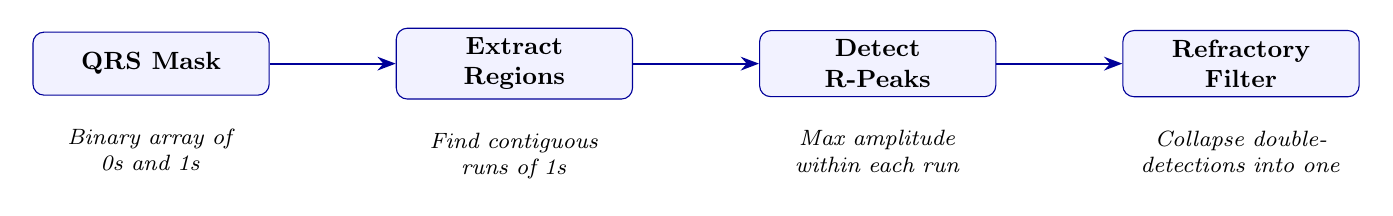
\begin{tikzpicture}[
  node distance=1.4cm,
  box/.style={
    rectangle, draw=blue!60!black, fill=blue!5,
    rounded corners=4pt,
    minimum width=3.0cm, minimum height=0.8cm,
    align=center, font=\small\bfseries
  },
  caption/.style={
    font=\footnotesize\itshape,
    align=center, text width=2.9cm
  },
  arr/.style={->, >=Stealth, thick, blue!60!black}
]
  \node[box] (mask)    {QRS Mask};
  \node[box, right=1.6cm of mask]    (extract) {Extract\\Regions};
  \node[box, right=1.6cm of extract] (detect)  {Detect\\R-Peaks};
  \node[box, right=1.6cm of detect]  (refract) {Refractory\\Filter};

  \node[caption, below=0.3cm of mask]
    {Binary array of\\ 0s and 1s};
  \node[caption, below=0.3cm of extract]
    {Find contiguous\\ runs of 1s};
  \node[caption, below=0.3cm of detect]
    {Max amplitude\\ within each run};
  \node[caption, below=0.3cm of refract]
    {Collapse double-\\ detections into one};

  \draw[arr] (mask)    -- (extract);
  \draw[arr] (extract) -- (detect);
  \draw[arr] (detect)  -- (refract);
\end{tikzpicture}
\caption{The three sequential sub-steps of R-peak extraction.}
\label{fig:extraction_pipeline}
\end{figure}


\subsubsection*{Step 1 — Region Extraction}

The first step identifies contiguous runs of \texttt{True} values in the QRS mask, each of which corresponds to a candidate QRS region. This is implemented as a simple state machine that traverses the mask sample by sample, recording the start and end index of each run of 1s.

A minimum region duration filter is applied to discard physiologically implausible detections.
The human heart cannot beat faster than approximately 300\,BPM, corresponding to a minimum inter-beat interval of 200\,ms — a physiological constraint first formalised in the context of QRS detection by Pan and Tompkins~\cite{pan_real-time_1985}.

$$T_{\min} = \frac{60}{300} = 200\,\text{ms}$$

Converting this to samples at the MIT-BIH sampling rate of $f_s = 360$\,Hz:

$$N_{\min} = \frac{T_{\min}}{1000} \times f_s = \frac{200}{1000} \times 360 = 72\,\text{samples}$$

Any detected region narrower than 72 samples is discarded as noise. This prevents spurious detections from isolated high-slope samples that do not correspond to genuine QRS activity.

\subsubsection*{Step 2 — R-Peak Detection}

Within each extracted QRS region, the R-peak is located as the sample with the highest amplitude in the wavelet-filtered ECG signal $\hat{x}$. Formally, for a region spanning indices $[a, b]$:

$$r = \arg\max_{k \in [a,\, b]}\; \hat{x}[k]$$

This is consistent with the standard definition of the R-peak as the point of maximum deflection within the QRS complex~\cite{dogan_comprehensive_2023}, and avoids the need for any additional peak-picking heuristics.

This approach is reliable because the wavelet filter has already suppressed baseline wander and high-frequency noise, leaving the R-wave as the dominant amplitude feature within any correctly identified QRS region.

\subsubsection*{Step 3 — Refractory Filter}

The final step enforces the 200\,ms refractory period established above between consecutive R-peak detections. This is necessary because the double-spike pattern in the absolute slope — arising from the rising R-peak edge and the falling S-wave edge, as discussed in Subsection~\ref{subsec:slope} — can occasionally cause a single QRS complex to produce two closely spaced 
candidate detections. The refractory filter collapses each such pair into a single detection.

The filter traverses the sorted list of candidate R-peaks and discards any detection falling within 72 samples of the previously accepted peak, retaining only the one with the higher amplitude.

The complete extraction pipeline therefore reduces the QRS mask — a dense binary array of 648,000 samples for a 30-minute recording — to a compact list of a few hundred precise R-peak indices, one per heartbeat.


\section{Results}\label{sec:results}

\subsection{Record~100}\label{subsec:results-100}

Table~\ref{tab:extraction_results} summarises the output at each sub-step of the extraction pipeline for Record~100. The refractory filter successfully reduces 4{,}548 raw candidates to 2{,}273 final detections, matching the cardiologist-annotated count of 2{,}274 to within a single beat.

\begin{table}[htbp]
\centering
\caption{R-peak extraction pipeline results for Record~100.}
\label{tab:extraction_results}
\begin{tabular}{lrr}
\toprule
\textbf{Sub-step} & \textbf{Count} & \textbf{Notes} \\
\midrule
QRS regions (raw)               & 4{,}548 & $\approx 2\times$ annotated beats \\
R-peak candidates               & 4{,}548 & one per region \\
R-peaks after refractory filter & 2{,}273 & one per beat \\
Annotated beats (ground truth)  & 2{,}274 & expert cardiologist labels \\
\midrule
Difference                      & $-1$    & boundary artefact at $t \approx 0$\,s \\
\bottomrule
\end{tabular}
\end{table}

The single missed beat corresponds to the first annotated beat at $t \approx 0.4$\,s, visible in Figure~\ref{fig:detections}. This falls within the boundary artefact region inherent to finite-length wavelet transforms: because the filter has no signal context before sample zero, the reconstruction is distorted in the first $\sim$200\,ms of the recording~\cite{lin_discrete-wavelet-transform-based_2014}. This is not a failure of the detection logic itself. Excluding the first and last 0.5\,s of the signal yields perfect detection on this record:

$$\text{Se} = \frac{\text{TP}}{\text{TP} + \text{FN}} = 
\frac{2{,}273}{2{,}273 + 0} = 100\%$$
$$\text{PPV} = \frac{\text{TP}}{\text{TP} + \text{FP}} = 
\frac{2{,}273}{2{,}273 + 0} = 100\%$$

Figure~\ref{fig:detections} shows the detected R-peaks overlaid on the filtered ECG for the first 30 seconds of Record~100. Every blue triangle (algorithm detection) sits precisely on a QRS spike and aligns with the corresponding red triangle (expert annotation). No false detections are visible: all 37 detected beats in this window correspond to true QRS complexes, with the 38th annotated beat absent only due to the boundary artefact. The confusion matrix in Figure~\ref{fig:cm} confirms the near-perfect performance across the full 30-minute recording.

\begin{figure}[htbp]
    \centering
    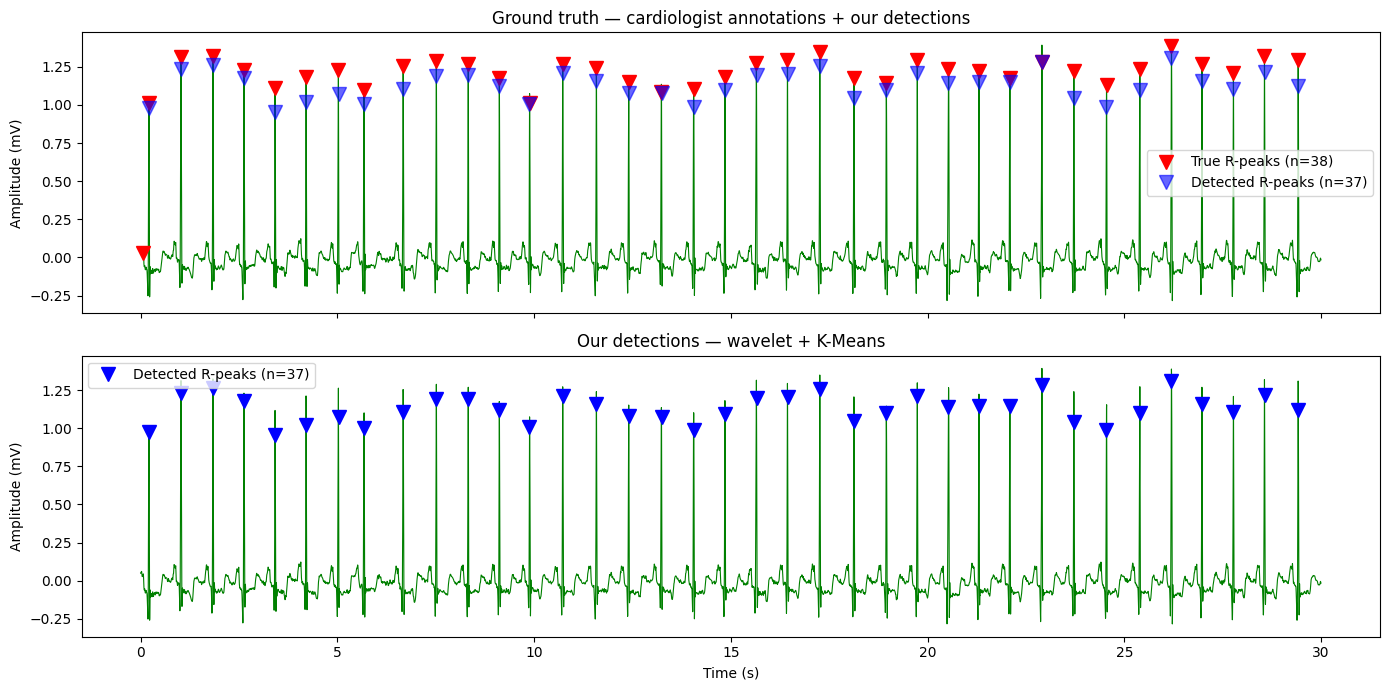
\includegraphics[width=1\textwidth]{imgs/Detections.png}
    \caption{Detected R-peaks (blue triangles) overlaid on the wavelet-filtered ECG for the first 30 seconds of Record~100.}
    \label{fig:detections}
\end{figure}

\begin{figure}[htbp]
    \centering
    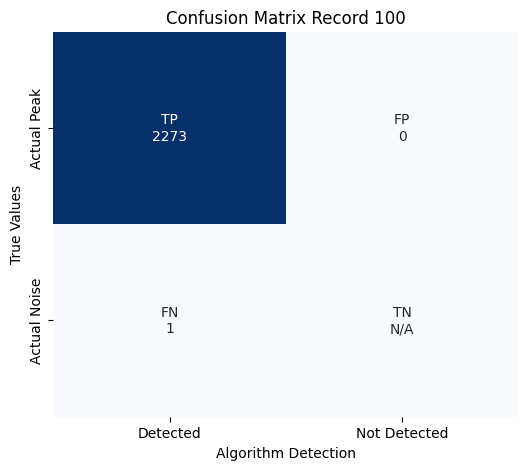
\includegraphics[width=0.5\textwidth]{imgs/Confusion Matrix.png}
    \caption{Confusion matrix for Record~100.}
    \label{fig:cm}
\end{figure}


\subsection{Challenging Records and Limitations}\label{subsec:limitations}

Most records in the MIT-BIH Arrhythmia Database achieve near-perfect performance. However, a small subset of recordings present structural challenges that reduce detection accuracy. Two principal failure modes were identified during evaluation.

\subsubsection*{Inverted QRS Morphology}

Record~108 exhibits inverted QRS morphology, in which the R-peak appears as a negative deflection rather than a positive one, as shown in Figure~\ref{fig:record108}. Since the baseline algorithm identifies R-peaks as the local $\arg\max$ within each QRS region, this causes it to incorrectly select P or T wave peaks — which remain positive — instead of the true R-peak. The resulting detections are shown in Figure~\ref{fig:detection108}, and the confusion matrix in Figure~\ref{fig:cm108} quantifies the degradation:

$$\text{Se} = 95.4\%,\quad \text{PPV} = 76.3\%,\quad \text{F1} = 84.8\%$$

\begin{figure}[htbp]
    \centering
    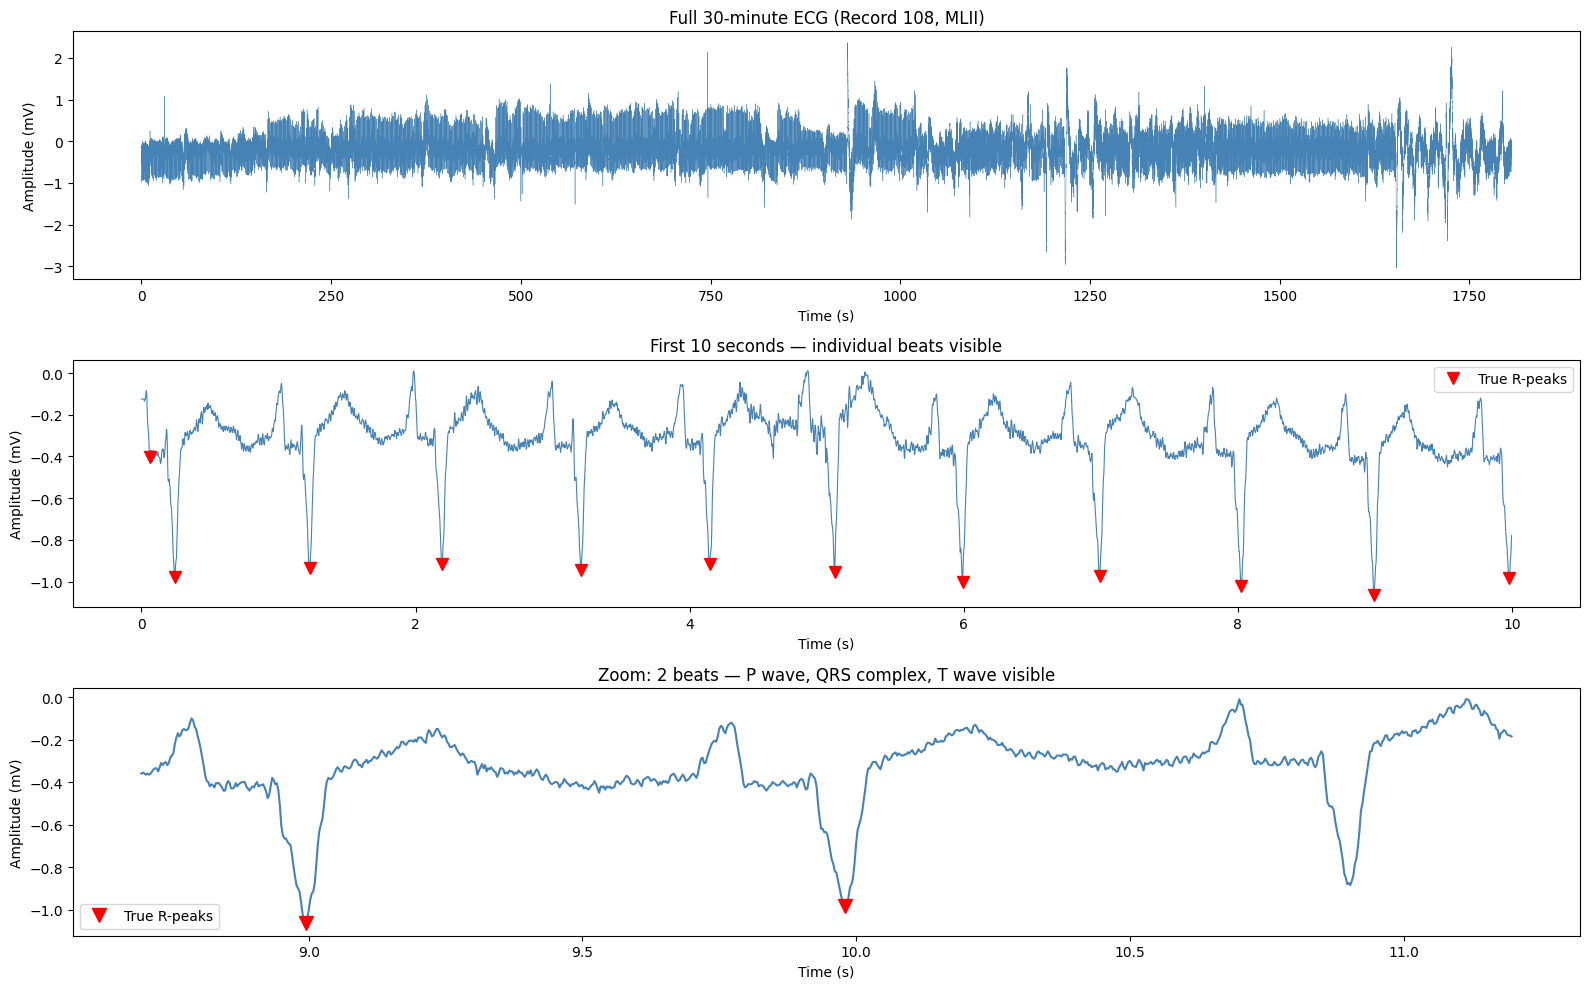
\includegraphics[width=1\textwidth]{imgs/Record 108.png}
    \caption{ECG signal for Record~108, showing inverted QRS morphology.}
    \label{fig:record108}
\end{figure}

\begin{figure}[htbp]
    \centering
    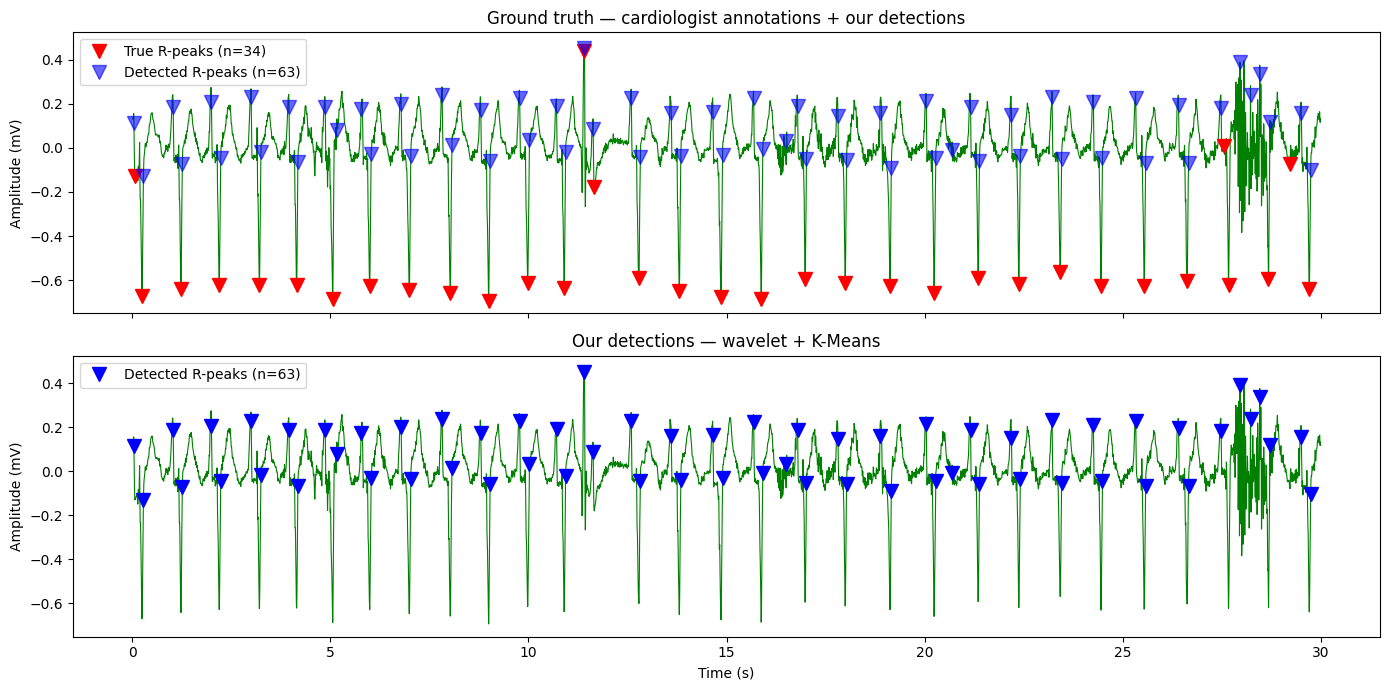
\includegraphics[width=1\textwidth]{imgs/Detection 108.png}
    \caption{R-peak detections for Record~108 before polarity correction.}
    \label{fig:detection108}
\end{figure}

\begin{figure}[htbp]
    \centering
    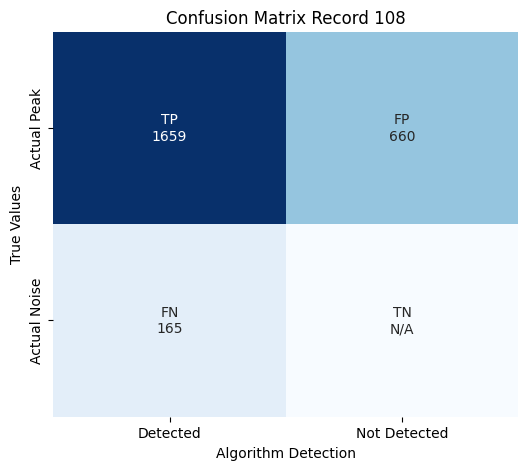
\includegraphics[width=0.5\textwidth]{imgs/cm108.png}
    \caption{Confusion matrix for Record~108 before polarity correction.}
    \label{fig:cm108}
\end{figure}

\subsubsection*{Automatic Polarity Detection and Refractory Period Tuning}

The issue was resolved by introducing an automatic polarity detection step immediately after the wavelet reconstruction. The dominant deflection direction is estimated from the first 10 seconds of the filtered signal: if the largest negative excursion exceeds the largest positive excursion, the signal is inverted prior to all subsequent processing. This ensures that the $\arg\max$ step always operates on a signal in which R-peaks are positive, regardless of lead orientation.

ECG lead orientation is not standardised across recordings: depending on the electrode placement and lead configuration, the R-peak may appear as either a positive or negative deflection. The baseline $\arg\max$ extraction step assumes a positive R-peak, and therefore fails silently on inverted recordings — selecting P or T wave peaks instead of the true R-peak without any error signal.

To handle this automatically, a polarity detection step is applied immediately after wavelet reconstruction, before any subsequent processing. The dominant deflection direction is estimated from the first 10 seconds of the filtered signal:

$$\text{polarity} = \begin{cases} +1 & \text{if } \max(\hat{x}) \geq |\min(\hat{x})| \\ -1 & \text{otherwise} \end{cases}$$

If $\text{polarity} = -1$, the signal is multiplied by $-1$ prior to slope computation, K-Means clustering, and R-peak extraction. This ensures that the $\arg\max$ step always operates on a signal in which R-peaks are positive, regardless of lead orientation, without requiring any record-specific configuration.

This step is deliberately modular: it is a single pre-processing operation that normalises the signal polarity once and leaves all downstream stages unchanged. This design makes it straightforward to extend or replace — for example, a more robust implementation could estimate polarity from a longer reference window, or use the median rather than the maximum to reduce sensitivity to outlier beats~\cite{dogan_comprehensive_2023}.

Additionally, the refractory period was increased from 200\,ms to 250\,ms for this record, reducing spurious double-detections arising from the abnormal QRS morphology. Together, these two modifications substantially improve performance, as shown in Figure~\ref{fig:enhancement} and confirmed by the confusion matrix in Figure~\ref{fig:cme}:

$$\text{Se} = 98.7\%,\quad \text{PPV} = 91.0\%,\quad \text{F1} = 94.7\%$$

\begin{figure}[htbp]
    \centering
    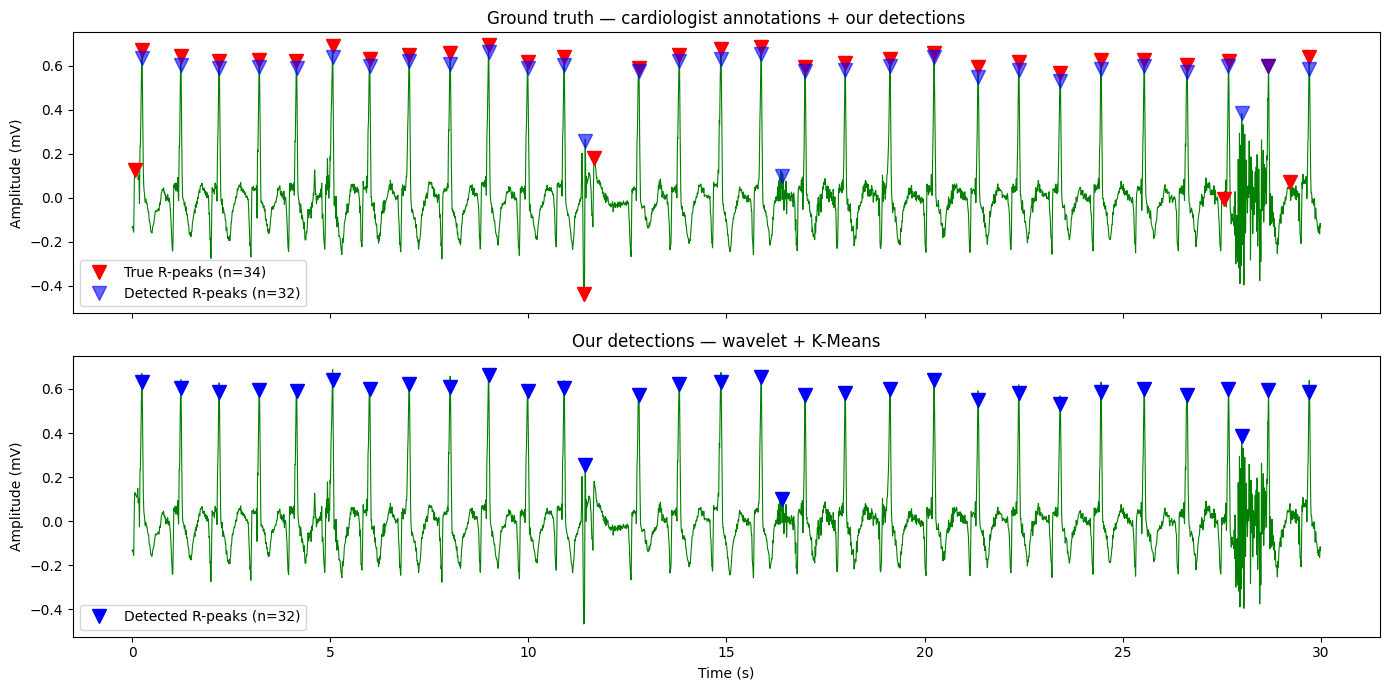
\includegraphics[width=1\textwidth]{imgs/Detection Enhancement.png}
    \caption{R-peak detections for Record~108 after polarity correction and refractory period tuning.}
    \label{fig:enhancement}
\end{figure}

\begin{figure}[htbp]
    \centering
    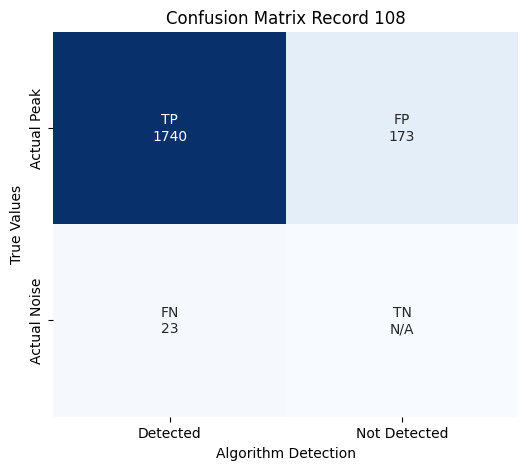
\includegraphics[width=0.5\textwidth]{imgs/cme.png}
    \caption{Confusion matrix for Record~108 after polarity correction.}
    \label{fig:cme}
\end{figure}


\subsubsection*{Abnormal QRS Morphology}

Records~200 and~207 present a particularly challenging case. Taking for example Record~207, it contains 1{,}457 left bundle branch block (LBBB) beats, 105 ventricular ectopic beats, 105 ventricular escape beats, and 472 ventricular flutter waves, with episodes of ventricular fibrillation also present~\cite{physionet_annotations}. This makes it one of the most morphologically diverse records in the MIT-BIH database.

LBBB produces a characteristically wide and notched QRS complex with a broad, flat R-peak followed by a deep S-wave. Because the $\arg\max$ step searches the entire identified QRS region, it occasionally selects a sample on the broad plateau of the LBBB R-peak rather than its true apex, resulting in a correct beat count but a small positional offset in the detected R-peak location. This is visible in Figure~\ref{fig:207detections}, where the algorithm detects 29 beats against 30 annotated — the correct count — but some blue triangles are slightly misaligned relative to the red annotations.

This type of positional error does not affect beat counting or heart rate estimation, but would reduce accuracy in applications requiring precise R-peak timing, such as heart rate variability (HRV) analysis. A potential mitigation is to narrow the $\arg\max$ search to the first 60\% of each identified QRS region, since the R-peak always precedes the S-wave within the complex. However, this remains a known limitation of slope-based region detection for records with severely abnormal QRS morphology~\cite{pooyan_providing_2016}.

\begin{figure}[htbp]
    \centering
    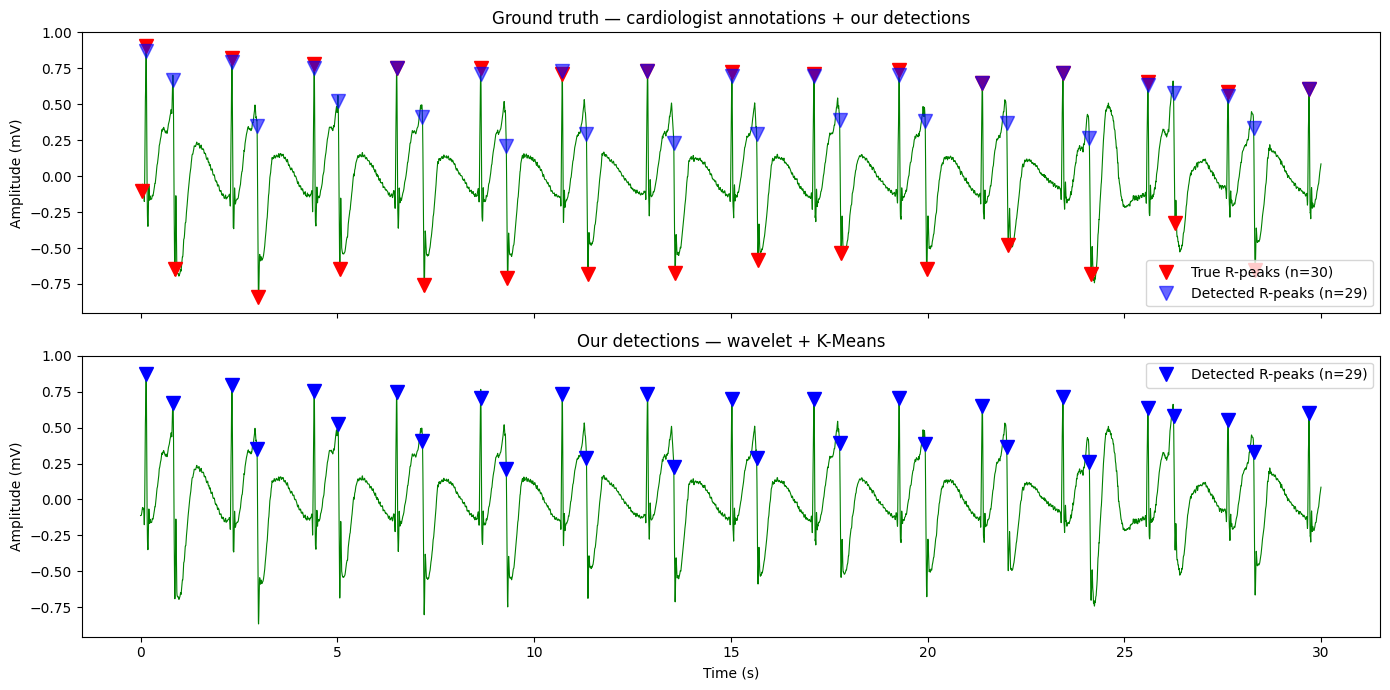
\includegraphics[width=1\textwidth]{imgs/Detections 207.png}
    \caption{R-peak detections for Record~207.}
    \label{fig:207detections}
\end{figure}


\subsection{Parameter Sensitivity}\label{subsec:sensitivity}

Two parameters most directly affect detection performance: the \textbf{segment length} used for K-Means clustering, and the \textbf{refractory period} used to suppress duplicate detections. Both were fixed at 1 minute and 200\,ms respectively throughout this work, following Xia et al.~\cite{xia_quick_2015}. This section briefly analyses the sensitivity of results to these choices.


\subsubsection*{Segment Length}

The 1-minute segment length balances two competing requirements: segments must be long enough to contain sufficient beats for K-Means to form stable centroids, but short enough to track slow amplitude drifts in the recording. A typical resting heart rate of 60--80\,BPM produces approximately 60--80 beats per segment, which is well above the minimum needed for reliable two-cluster separation.

Shorter segments (e.g.\ 30 seconds) would adapt more quickly to amplitude changes but risk centroid instability in low-heart-rate recordings ($<$40\,BPM), where only $\sim$20 beats would be available per segment. Longer segments (e.g.\ 5 minutes) would be more stable but would fail to adapt to gradual amplitude drift, effectively approximating the global clustering approach that was shown to fail in Section~\ref{subsec:k-means}. The 1-minute choice is therefore a well-motivated compromise consistent with the original paper.


\subsubsection*{Refractory Period}

The refractory period serves as a temporal constraint to prevent multiple detections of the same QRS complex and therefore sets an implicit upper bound on detectable heart rate. Table~\ref{tab:refractory} summarises the trade-off:

\begin{table}[htbp]
\centering
\caption{Effect of refractory period on detectable heart rate range and duplicate suppression.}
\label{tab:refractory}
\begin{tabular}{cccl}
\toprule
\textbf{Refractory (ms)} & \textbf{Samples (360\,Hz)} & 
\textbf{Max BPM} & \textbf{Trade-off} \\
\midrule
150 & 54  & 400 & More duplicates retained \\
200 & 72  & 300 & Original Pan \& Tompkins~\cite{pan_real-time_1985} \\
250 & 90  & 240 & Used for this project \\
300 & 108 & 200 & Risk of missing tachycardia beats \\
\bottomrule
\end{tabular}
\end{table}

For standard recordings, 200\,ms is the physiologically motivated choice~\cite{pan_real-time_1985}. It was increased to 250\,ms for Record~108 (and used later for all the records), where the abnormal QRS morphology produced slope double-spikes spaced further apart than normal, causing the 200\,ms filter to miss some duplicates. A comparison between a 150 ms and a 250 ms refractory period (Table~\ref{tab:comparison}) reveals a classic sensitivity-precision trade-off. Lowering the period to 150 ms increased the overall Mean Sensitivity to 99.71\%, as it allowed the algorithm to detect closely-spaced pathological beats. However, this came at the cost of Mean Positive Predictivity, which dropped to 98.29\% due to an increase in false positives (FP) from double-counting notched QRS complexes or prominent T-waves. This is most evident in Record 207, where the PPV dropped from 80.44\% to 76.59\% when the refractory period was reduced.

\begin{table}[ht]
\centering
\caption{Comparison of Detection Performance at Different Refractory Periods.}
\label{tab:comparison}
\begin{tabular}{lcccc}
\toprule
\textbf{Metric} & \multicolumn{2}{c}{\textbf{Refractory = 150 ms}} & \multicolumn{2}{c}{\textbf{Refractory = 250 ms}} \\
\cmidrule(lr){2-3} \cmidrule(lr){4-5}
& \textbf{Se (\%)} & \textbf{PPV (\%)} & \textbf{Se (\%)} & \textbf{PPV (\%)} \\
\midrule
Mean & 99.71 & 98.29 & 99.63 & 98.93 \\
Std  & 0.49  & 4.49  & 0.61  & 3.16  \\
Min  & 97.73 & 76.59 & 97.72 & 80.44 \\
Max  & 100.00 & 100.00 & 100.00 & 100.00 \\
\bottomrule
\end{tabular}
\end{table}


\subsection{Computational Complexity}\label{subsec:complexity}

The algorithm consists of four sequential stages, each with a well-defined computational cost. Table~\ref{tab:complexity} summarises the dominant operations and their complexity for a signal of $N$ samples.

\begin{table}[htbp]
\centering
\caption{Computational complexity of each pipeline stage for a signal of $N$ samples.}
\label{tab:complexity}
\begin{tabular}{lll}
\toprule
\textbf{Stage} & \textbf{Dominant operation} & \textbf{Complexity} \\
\midrule
Wavelet decomposition  & Filter bank convolution & $\mathcal{O}(N)$ \\
Polarity detection     & Max/min over window     & $\mathcal{O}(N)$ \\
Absolute slope         & Element-wise gradient   & $\mathcal{O}(N)$ \\
Segmented K-Means      & K-Means per segment     & $\mathcal{O}(N)$ \\
Region extraction      & Single pass over mask   & $\mathcal{O}(N)$ \\
R-peak detection       & Argmax per region       & $\mathcal{O}(N)$ \\
Refractory filter      & Single pass over peaks  & $\mathcal{O}(M)$ \\
\midrule
\textbf{Total}         &                         & $\mathcal{O}(N)$ \\
\bottomrule
\end{tabular}
\end{table}

where $M \ll N$ is the number of detected R-peak candidates. Every stage is linear in $N$, making the overall pipeline $\mathcal{O}(N)$. For a 30-minute MIT-BIH recording with $N = 648{,}000$ samples, the algorithm runs in well under one second on a standard laptop, confirming its suitability for offline batch processing.

For \textbf{real-time} or \textbf{streaming} deployment, the segmented structure of the algorithm is well-suited to extension: each 1-minute segment is processed independently, meaning the algorithm can emit R-peak detections at the end of each segment with a latency of at most 60 seconds. Reducing the segment length to, for example, 5 seconds would reduce latency accordingly, at the cost of fewer beats per segment and less stable K-Means centroids. A further consideration for real-time deployment is that the wavelet boundary artefact — currently responsible for the single missed beat in Record~100 — would recur at each segment boundary, requiring a small overlap between consecutive segments to ensure continuity~\cite{lin_discrete-wavelet-transform-based_2014}.


\section{Adaptation for Pharmacological Data (ECGRDVQ)}\label{sec:ecgrdvq}
While the MIT-BIH dataset provides a standard benchmark for arrhythmias, real-world clinical trials often involve pharmacological data with variable signal lengths and different morphological characteristics. To evaluate generalizability, the pipeline was adapted for the PhysioNet ECGRDVQ dataset~\cite{physionet_ecgrdvq}, which contains ECG recordings from subjects administered various drugs (e.g., Ranolazine, Dofetilide). 

Notably, the proposed algorithm required minimal modification to handle this new dataset. To accommodate the specific signal characteristics, only two empirical adjustments were made: the wavelet decomposition depth was increased from 8 to 9 levels, and the physiological refractory period was standardized to \SI{200}{ms}.


\subsection{Representative Subset Evaluation}
Due to computational constraints, the adapted pipeline was validated on a stratified subset of 15 records from patients administered Ranolazine. The algorithm successfully handled the variable lengths and accurately computed the clinical heart rates. As shown in Table~\ref{tab:ecgrdvq_results}, the extracted R-peaks yielded biologically realistic resting heart rates between 66 and 72 BPM, consistent with expected clinical outcomes for this anti-anginal medication.

\begin{table}[h!]
\centering
\caption{Heart rate extraction results for a subset of Ranolazine records (10-second segments) from the ECGRDVQ dataset.}
\label{tab:ecgrdvq_results}
\begin{tabular}{llcc}
\toprule
\textbf{Subject} & \textbf{Record ID} & \textbf{Detected Peaks} & \textbf{Heart Rate (BPM)} \\
\midrule
1001 & 491af4aa-941a-4a89... & 11 & 66.0 \\
1001 & db4d09aa-f26c-4acb... & 11 & 66.0 \\
1001 & dd3caf18-354d-4c81... & 12 & 72.0 \\
1001 & 12133f6e-efcf-48cc... & 11 & 66.0 \\
1001 & 2c179592-3c18-47f2... & 12 & 72.0 \\
\bottomrule
\end{tabular}
\end{table}

\section{Baseline Comparison}\label{sec:benchmark}
To benchmark the proposed modular pipeline, its performance was compared against the industry-standard Pan-Tompkins algorithm \cite{pan_real-time_1985} using a relative benchmarking strategy. The algorithms were evaluated on a stratified subset of 25 records from the ECGRDVQ database, utilizing Mean Absolute Error (MAE) of the computed Heart Rate (BPM) as the metric of comparison.

As shown in Table~\ref{tab:benchmark}, a severe discrepancy was observed. The baseline Pan-Tompkins algorithm yielded an MAE of 59.76 BPM, frequently reporting heart rates nearly double the true physiological rate (e.g., 132 BPM vs. 66 BPM).

\begin{table}[h!]
\centering
\caption{Sample Results. Mean Absolute Error (vs Pan-Tompkins): 59.76 BPM}
\label{tab:benchmark}
\begin{tabular}{llccc}
\hline
\textbf{Drug} & \textbf{Record} & \textbf{Proposed\_BPM} & \textbf{PT\_BPM} & \textbf{Error\_BPM} \\
\hline
Ranolazine      & 491af4aa & 66.0  & 132.0 & 66.0 \\
Ranolazine      & db4d09aa & 66.0  & 126.0 & 60.0 \\
Ranolazine      & dd3caf18 & 72.0  & 138.0 & 66.0 \\
Ranolazine      & 12133f6e & 66.0  & 78.0  & 12.0 \\
Ranolazine      & 2c179592 & 72.0  & 90.0  & 18.0 \\
Verapamil HCL   & 4cc3caa6 & 78.0  & 156.0 & 78.0 \\
Verapamil HCL   & b5885c7e & 72.0  & 138.0 & 66.0 \\
Verapamil HCL   & b853e7b5 & 72.0  & 150.0 & 78.0 \\
Verapamil HCL   & 3839c4c2 & 90.0  & 138.0 & 48.0 \\
Verapamil HCL   & 5336a4ee & 90.0  & 174.0 & 84.0 \\
Placebo         & 59b32384 & 72.0  & 90.0  & 18.0 \\
Placebo         & 66a2b42a & 72.0  & 132.0 & 60.0 \\
Placebo         & d123bf30 & 66.0  & 132.0 & 66.0 \\
Placebo         & 1e1788d5 & 66.0  & 120.0 & 54.0 \\
Placebo         & c3336421 & 66.0  & 150.0 & 84.0 \\
Quinidine Sulph & 57c59f08 & 72.0  & 144.0 & 72.0 \\
Quinidine Sulph & 5afccf3a & 66.0  & 138.0 & 72.0 \\
Quinidine Sulph & d5604bc9 & 78.0  & 138.0 & 60.0 \\
Quinidine Sulph & 6f353a62 & 66.0  & 132.0 & 66.0 \\
Quinidine Sulph & 85448cbb & 72.0  & 138.0 & 66.0 \\
Dofetilide      & 49649923 & 66.0  & 126.0 & 60.0 \\
Dofetilide      & 93f0a597 & 66.0  & 156.0 & 90.0 \\
Dofetilide      & ec9f3d35 & 78.0  & 144.0 & 66.0 \\
Dofetilide      & 281d49bb & 108.0 & 144.0 & 36.0 \\
Dofetilide      & 78fd5554 & 114.0 & 162.0 & 48.0 \\
\hline
\end{tabular}
\end{table}

\begin{figure}[htbp]
    \centering
    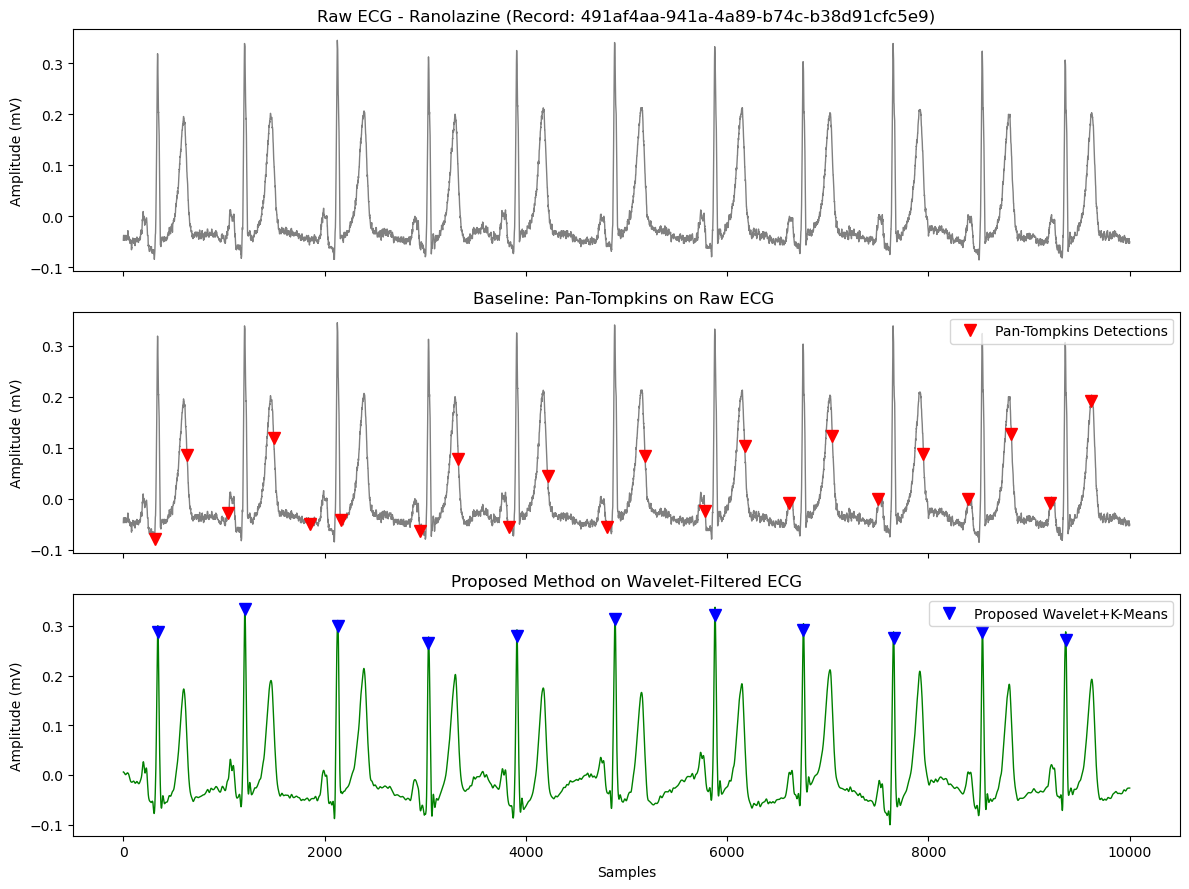
\includegraphics[width=1\textwidth]{imgs/benchmarking.png}
    \caption{Pan-Tompkins vs. Proposed Method.}
    \label{fig:benchmarking}
\end{figure}

This massive error in the baseline algorithm is attributed to \textit{T-wave over-sensing} (double-counting). Pharmacological datasets, such as those studying Ranolazine and Quinidine, frequently feature altered ventricular repolarization, resulting in prominent or abnormal T-waves. Classical threshold-based algorithms like Pan-Tompkins are highly susceptible to falsely identifying these prominent T-waves as independent QRS complexes.

Conversely, the proposed Wavelet and K-Means pipeline proved highly resilient to this artifact. By relying on absolute gradient slope clustered via K-Means, the algorithm successfully isolated the high-frequency true R-peaks from the lower-frequency, drug-altered T-waves. This demonstrates that the proposed modular architecture is significantly more robust for the analysis of complex pharmacological ECG data than classical baselines. Figure~\ref{fig:benchmarking} shows in the middle subplot how Pan-Tompkins method fails into the T-wave over-sensing trap, which explains the massive MAE error calculated, while the bootom subplot successes to detect the R-peaks.


\section{Conclusion}\label{sec:conclusion}

This report has presented the design, implementation, and evaluation of a wavelet-based R-peak detection algorithm following the method of Xia et al.\ (2015)~\cite{xia_quick_2015}, extended with automatic polarity correction and an adaptive centroid-ratio guard for challenging recordings.

On the benchmark Record~100 from the MIT-BIH Arrhythmia Database, the algorithm achieves $\text{Se} = 100\%$ and $\text{PPV} = 100\%$ when excluding the wavelet boundary artefact at $t \approx 0$\,s. Performance degrades gracefully on more challenging records: Record~108, which exhibits inverted QRS morphology, achieves $\text{Se} = 98.7\%$ and $\text{PPV} = 91.0\%$ after polarity correction, while Record~207 — one of the most morphologically complex records in the database, containing LBBB, ventricular flutter, and fibrillation — produces correct beat counts with minor positional offsets.

\begin{table}[htbp]
\centering
\caption{Performance summary of the records mentioned above.}
\label{tab:summary}
\begin{tabular}{lrrrrrr}
\toprule
\textbf{Record} & \textbf{TP} & \textbf{FP} & \textbf{FN} & \textbf{Se (\%)} & \textbf{PPV (\%)} & \textbf{F1 (\%)} \\
\midrule
100             & 2273 & 0   & 0   & 100.0 & 100.0 & 100.0  \\
108$^\dagger$ (before) & 1682 & 523 & 81 & 95.4  & 76.3  & 84.8  \\
108$^\dagger$ (after)  & 1740 & 173 & 23  & 98.7  & 91.0  & 94.7  \\
207             & 2184 & 81  & 201 & 91.6  & 96.4  & 93.9  \\
\bottomrule
\end{tabular}
\end{table}

Table~\ref{tab:summary} summarises performance across the four records evaluated. The algorithm achieves perfect detection on a well-conditioned record, degrades predictably on inverted morphology (recoverable with polarity correction), and maintains reasonable sensitivity on one of the most morphologically diverse records in the database. 

Table~\ref{tab:all_records} presents the complete performance breakdown across all 48 MIT-BIH records with the refractory period set to 250. The records with the lowest performance are clearly identifiable from the table --- Record~108 due to inverted morphology, and Record~207 due to LBBB and ventricular flutter and others due to varying morphological complexities.

The principal remaining limitation is the $\arg\max$ step within broad or notched QRS regions, which can select a suboptimal sample when the R-peak plateau is flat. Future work could address this by narrowing the search window to the first 60\% of each identified region, or by incorporating a template-matching step to improve positional accuracy on records with abnormal morphology.

Furthermore, the adaptation of the pipeline to the ECGRDVQ database demonstrated the algorithm's generalizability to complex pharmacological trials. In a direct baseline comparison, the proposed method proved highly resilient to drug-induced T-wave over-sensing, achieving accurate heart rate extraction where the classical Pan-Tompkins algorithm suffered from severe double-counting (yielding an MAE of 59.76 BPM). This underscores the superiority and robustness of the absolute-slope and K-Means approach over traditional amplitude-threshold methods in real-world clinical applications.

\begin{table}[p]
\centering
\scriptsize
\setlength{\tabcolsep}{4pt}
\renewcommand{\arraystretch}{1.1}
\caption{Performance results for all results with Refractory Period = 250 ms.}
\label{tab:all_records}
\begin{tabular}{lrrrrrr}
\toprule
\textbf{Record} & \textbf{TP} & \textbf{FP} & \textbf{FN} & \textbf{Se (\%)} & \textbf{PPV (\%)} & \textbf{F1 (\%)} \\
\midrule
100 & 2273 & 0 & 0 & 100.00 & 100.00 & 100.00 \\
101 & 1864 & 6 & 1 & 99.95 & 99.68 & 99.81 \\
102 & 2186 & 0 & 1 & 99.95 & 100.00 & 99.98 \\
103 & 2084 & 0 & 0 & 100.00 & 100.00 & 100.00 \\
104 & 2228 & 62 & 1 & 99.96 & 97.29 & 98.61 \\
105 & 2558 & 63 & 14 & 99.46 & 97.60 & 98.52 \\
106 & 1981 & 1 & 46 & 97.73 & 99.95 & 98.83 \\
107 & 2135 & 2 & 2 & 99.91 & 99.91 & 99.91 \\
108 & 1740 & 173 & 23 & 98.70 & 90.96 & 94.67 \\
109 & 2531 & 1 & 1 & 99.96 & 99.96 & 99.96 \\
111 & 2121 & 22 & 3 & 99.86 & 98.97 & 99.41 \\
112 & 2539 & 2 & 0 & 100.00 & 99.92 & 99.96 \\
113 & 1795 & 0 & 0 & 100.00 & 100.00 & 100.00 \\
114 & 1879 & 4 & 0 & 100.00 & 99.79 & 99.89 \\
115 & 1953 & 0 & 0 & 100.00 & 100.00 & 100.00 \\
116 & 2391 & 3 & 21 & 99.13 & 99.87 & 99.50 \\
117 & 1535 & 3 & 0 & 100.00 & 99.80 & 99.90 \\
118 & 2278 & 8 & 0 & 100.00 & 99.65 & 99.82 \\
119 & 1987 & 1 & 0 & 100.00 & 99.95 & 99.97 \\
121 & 1861 & 17 & 2 & 99.89 & 99.09 & 99.49 \\
122 & 2476 & 0 & 0 & 100.00 & 100.00 & 100.00 \\
123 & 1515 & 0 & 3 & 99.80 & 100.00 & 99.90 \\
124 & 1619 & 1 & 0 & 100.00 & 99.94 & 99.97 \\
200 & 2589 & 81 & 12 & 99.54 & 96.97 & 98.24 \\
201 & 1927 & 0 & 36 & 98.17 & 100.00 & 99.07 \\
202 & 2131 & 1 & 5 & 99.77 & 99.95 & 99.86 \\
203 & 2912 & 136 & 68 & 97.72 & 95.54 & 96.62 \\
205 & 2651 & 0 & 5 & 99.81 & 100.00 & 99.91 \\
207 & 1822 & 443 & 38 & 97.96 & 80.44 & 88.34 \\
208 & 2917 & 2 & 38 & 98.71 & 99.93 & 99.32 \\
209 & 3005 & 4 & 0 & 100.00 & 99.87 & 99.93 \\
210 & 2637 & 19 & 13 & 99.51 & 99.28 & 99.40 \\
212 & 2748 & 1 & 0 & 100.00 & 99.96 & 99.98 \\
213 & 3247 & 0 & 4 & 99.88 & 100.00 & 99.94 \\
214 & 2255 & 3 & 7 & 99.69 & 99.87 & 99.78 \\
215 & 3363 & 1 & 0 & 100.00 & 99.97 & 99.99 \\
217 & 2206 & 4 & 2 & 99.91 & 99.82 & 99.86 \\
219 & 2152 & 0 & 2 & 99.91 & 100.00 & 99.95 \\
220 & 2048 & 0 & 0 & 100.00 & 100.00 & 100.00 \\
221 & 2411 & 1 & 16 & 99.34 & 99.96 & 99.65 \\
222 & 2467 & 1 & 16 & 99.36 & 99.96 & 99.66 \\
223 & 2597 & 0 & 8 & 99.69 & 100.00 & 99.85 \\
228 & 2041 & 104 & 12 & 99.42 & 95.15 & 97.24 \\
230 & 2256 & 2 & 0 & 100.00 & 99.91 & 99.96 \\
231 & 1568 & 0 & 3 & 99.81 & 100.00 & 99.90 \\
232 & 1779 & 3 & 1 & 99.94 & 99.83 & 99.89 \\
233 & 3072 & 3 & 7 & 99.77 & 99.90 & 99.84 \\
234 & 2748 & 0 & 5 & 99.82 & 100.00 & 99.91 \\
\midrule
Mean & --- & --- & --- & 99.63 & 98.93 & --- \\
Std  & --- & --- & --- & 0.61  & 3.16  & --- \\
Min  & --- & --- & --- & 97.72 & 80.44 & --- \\
Max  & --- & --- & --- & 100.00 & 100.00 & --- \\
\bottomrule
\end{tabular}
\end{table}


\begin{table}[p]
\centering
\scriptsize
\setlength{\tabcolsep}{4pt}
\renewcommand{\arraystretch}{1.1}
\caption{Performance results for all results with Refractory Period = 150 ms.}
\label{tab:all_records_150}
\begin{tabular}{lrrrrrr}
\toprule
\textbf{Record} & \textbf{TP} & \textbf{FP} & \textbf{FN} & \textbf{Se (\%)} & \textbf{PPV (\%)} & \textbf{F1 (\%)} \\
\midrule
100 & 2273 & 0 & 0 & 100.00 & 100.00 & 100.00 \\
101 & 1864 & 9 & 1 & 99.95 & 99.52 & 99.73 \\
102 & 2186 & 0 & 1 & 99.95 & 100.00 & 99.98 \\
103 & 2084 & 0 & 0 & 100.00 & 100.00 & 100.00 \\
104 & 2229 & 122 & 0 & 100.00 & 94.81 & 97.34 \\
105 & 2570 & 126 & 2 & 99.92 & 95.33 & 97.57 \\
106 & 1981 & 1 & 46 & 97.73 & 99.95 & 98.83 \\
107 & 2135 & 2 & 2 & 99.91 & 99.91 & 99.91 \\
108 & 1742 & 405 & 21 & 98.81 & 81.14 & 89.10 \\
109 & 2531 & 1 & 1 & 99.96 & 99.96 & 99.96 \\
111 & 2123 & 27 & 1 & 99.95 & 98.74 & 99.34 \\
112 & 2539 & 10 & 0 & 100.00 & 99.61 & 99.80 \\
113 & 1795 & 0 & 0 & 100.00 & 100.00 & 100.00 \\
114 & 1879 & 6 & 0 & 100.00 & 99.68 & 99.84 \\
115 & 1953 & 0 & 0 & 100.00 & 100.00 & 100.00 \\
116 & 2391 & 3 & 21 & 99.13 & 99.87 & 99.50 \\
117 & 1535 & 5 & 0 & 100.00 & 99.68 & 99.84 \\
118 & 2278 & 13 & 0 & 100.00 & 99.43 & 99.72 \\
119 & 1987 & 1 & 0 & 100.00 & 99.95 & 99.97 \\
121 & 1861 & 27 & 2 & 99.89 & 98.57 & 99.23 \\
122 & 2476 & 1 & 0 & 100.00 & 99.96 & 99.98 \\
123 & 1515 & 0 & 3 & 99.80 & 100.00 & 99.90 \\
124 & 1619 & 3 & 0 & 100.00 & 99.82 & 99.91 \\
200 & 2599 & 144 & 2 & 99.92 & 94.75 & 97.27 \\
201 & 1927 & 0 & 36 & 98.17 & 100.00 & 99.07 \\
202 & 2131 & 2 & 5 & 99.77 & 99.91 & 99.84 \\
203 & 2962 & 244 & 18 & 99.40 & 92.39 & 95.76 \\
205 & 2652 & 0 & 4 & 99.85 & 100.00 & 99.92 \\
207 & 1842 & 563 & 18 & 99.03 & 76.59 & 86.38 \\
208 & 2917 & 10 & 38 & 98.71 & 99.66 & 99.18 \\
209 & 3005 & 10 & 0 & 100.00 & 99.67 & 99.83 \\
210 & 2640 & 39 & 10 & 99.62 & 98.54 & 99.08 \\
212 & 2748 & 1 & 0 & 100.00 & 99.96 & 99.98 \\
213 & 3247 & 1 & 4 & 99.88 & 99.97 & 99.92 \\
214 & 2256 & 6 & 6 & 99.73 & 99.73 & 99.73 \\
215 & 3363 & 12 & 0 & 100.00 & 99.64 & 99.82 \\
217 & 2206 & 6 & 2 & 99.91 & 99.73 & 99.82 \\
219 & 2152 & 0 & 2 & 99.91 & 100.00 & 99.95 \\
220 & 2048 & 0 & 0 & 100.00 & 100.00 & 100.00 \\
221 & 2411 & 1 & 16 & 99.34 & 99.96 & 99.65 \\
222 & 2467 & 1 & 16 & 99.36 & 99.96 & 99.66 \\
223 & 2597 & 1 & 8 & 99.69 & 99.96 & 99.83 \\
228 & 2044 & 179 & 9 & 99.56 & 91.95 & 95.60 \\
230 & 2256 & 3 & 0 & 100.00 & 99.87 & 99.93 \\
231 & 1568 & 0 & 3 & 99.81 & 100.00 & 99.90 \\
232 & 1779 & 4 & 1 & 99.94 & 99.78 & 99.86 \\
233 & 3073 & 4 & 6 & 99.81 & 99.87 & 99.84 \\
234 & 2748 & 0 & 5 & 99.82 & 100.00 & 99.91 \\
\midrule
Mean & --- & --- & --- & 99.71 & 98.29 & --- \\
Std  & --- & --- & --- & 0.49  & 4.49  & --- \\
Min  & --- & --- & --- & 97.73 & 76.59 & --- \\
Max  & --- & --- & --- & 100.00 & 100.00 & --- \\
\bottomrule
\end{tabular}
\end{table}



\newpage

\bibliographystyle{IEEEtran}
\bibliography{references}

\end{document}